\documentclass[aspectratio=169, xcolor=dvipsnames]{beamer}
\usepackage{hyperref}
\usepackage[T1]{fontenc}

% Math packages
\usepackage {stmaryrd}
\usepackage{amsmath}
\usepackage{amssymb}
\usepackage{amsthm}
\usepackage{mathtools}
\usepackage{cancel}
\usepackage{ulem} % Strikeout in text mode
\usepackage{bbm} % mathbbm font for indicator function

% Algorithms and Code
\usepackage{algorithm, caption}
\usepackage{algorithmic}
\usepackage{listings}

% Graphics
\usepackage{latexsym,multicol,booktabs}
\usepackage{graphicx,pstricks,stackengine}
\usepackage{tikz}
\usetikzlibrary{positioning,arrows.meta, patterns, patterns.meta}
\usetikzlibrary{overlay-beamer-styles}
\usetikzlibrary{shapes,backgrounds} % Ellipses
\usetikzlibrary{decorations.pathreplacing,calligraphy} % Decorations (like braces)
\usetikzlibrary{calc} % Coordinate additions

% Custom colors
\definecolor{rwth-blue}{cmyk}{1,.5,0,0}\colorlet{rwth-lblue}{rwth-blue!50}\colorlet{rwth-llblue}{rwth-blue!25}
\definecolor{rwth-violet}{cmyk}{.6,.6,0,0}\colorlet{rwth-lviolet}{rwth-violet!50}\colorlet{rwth-llviolet}{rwth-violet!25}
\definecolor{rwth-purple}{cmyk}{.7,1,.35,.15}\colorlet{rwth-lpurple}{rwth-purple!50}\colorlet{rwth-llpurple}{rwth-purple!25}
\definecolor{rwth-carmine}{cmyk}{.25,1,.7,.2}\colorlet{rwth-lcarmine}{rwth-carmine!50}\colorlet{rwth-llcarmine}{rwth-carmine!25}
\definecolor{rwth-red}{cmyk}{.15,1,1,0}\colorlet{rwth-lred}{rwth-red!50}\colorlet{rwth-llred}{rwth-red!25}
\definecolor{rwth-magenta}{cmyk}{0,1,.25,0}\colorlet{rwth-lmagenta}{rwth-magenta!50}\colorlet{rwth-llmagenta}{rwth-magenta!25}
\definecolor{rwth-orange}{cmyk}{0,.4,1,0}\colorlet{rwth-lorange}{rwth-orange!50}\colorlet{rwth-llorange}{rwth-orange!25}
\definecolor{rwth-yellow}{cmyk}{0,0,1,0}\colorlet{rwth-lyellow}{rwth-yellow!50}\colorlet{rwth-llyellow}{rwth-yellow!25}
\definecolor{rwth-grass}{cmyk}{.35,0,1,0}\colorlet{rwth-lgrass}{rwth-grass!50}\colorlet{rwth-llgrass}{rwth-grass!25}
\definecolor{rwth-green}{cmyk}{.7,0,1,0}\colorlet{rwth-lgreen}{rwth-green!50}\colorlet{rwth-llgreen}{rwth-green!25}
\definecolor{rwth-cyan}{cmyk}{1,0,.4,0}\colorlet{rwth-lcyan}{rwth-cyan!50}\colorlet{rwth-llcyan}{rwth-cyan!25}
\definecolor{rwth-teal}{cmyk}{1,.3,.5,.3}\colorlet{rwth-lteal}{rwth-teal!50}\colorlet{rwth-llteal}{rwth-teal!25}
\definecolor{rwth-olive}{cmyk}{1,0,1,.4}\colorlet{rwth-lolive}{rwth-olive!50}\colorlet{rwth-llolive}{rwth-olive!25}
\definecolor{rwth-gold}{cmyk}{.35,.46,.7,.35}
\definecolor{rwth-silver}{cmyk}{.39,.31,.32,.14}
\definecolor{rwth-storm}{cmyk}{0.5,0.15,0,0.2}

%% COLORS SUITABLE WITH TSINGHUA PURPLE
% rwth-teal
% rwth-olive
% rwth-storm (Steel Blue)
% MidnightBlue
% Mahogany

% Typography
\newcommand\tab[1][1cm]{\hspace*{#1}}
\newcommand{\tabitem}{~~$\bullet$~~}
\newcommand{\bulletpoint}{\tab[0.5cm] \tabitem}
\newcommand{\arrowr}{$\bm{\rightarrow}$ }
\newcommand{\arrowrgreen}{{\color{rwth-green}\arrowr}}
\newcommand{\arrowrorange}{{\color{Orange}\arrowr}}
\newcommand{\proplus}{{\color{rwth-green}$\bm{\bigoplus}$} }
\newcommand{\concross}{{\color{Orange}$\bm{\bigotimes}$} }
\newcommand{\warning}{{\color{Orange}\textbf{!}} }

\author{Lukas R\"uttgers}
\title{Kolmogorov Complexity and How it Illuminates our Limitations to Let Machines Learn Simple Functions}
\subtitle{}
\institute{IIIS, Tsinghua University}
\date{\today}
\usepackage{Tsinghua}

% defs
\def\cmd#1{\texttt{\color{red}\footnotesize $\backslash$#1}}
\def\env#1{\texttt{\color{blue}\footnotesize #1}}
\definecolor{deepblue}{rgb}{0,0,0.5}
\definecolor{deepred}{rgb}{0.6,0,0}
\definecolor{deepgreen}{rgb}{0,0.5,0}
\definecolor{halfgray}{gray}{0.55}

\lstset{
	basicstyle=\ttfamily\small,
	keywordstyle=\bfseries\color{deepblue},
	emphstyle=\ttfamily\color{deepred},    % Custom highlighting style
	stringstyle=\color{deepgreen},
	numbers=left,
	numberstyle=\small\color{halfgray},
	rulesepcolor=\color{red!20!green!20!blue!20},
	frame=shadowbox,
}

% Customized commands
\newcommand{\llrrbracket}[1]{% \llrrbracket{..}
	\left[\mkern-3mu\left[#1\right]\mkern-3mu\right]}
\newcommand{\llrrparen}[1]{% \llrrparen{..}
	\left(\mkern-6mu\left(#1\right)\mkern-6mu\right)}
\algsetup{indent=1em, linenosize=\tiny}

\newcommand{\tikzxmark}{%
	\tikz[scale=0.23,draw=Mahogany] {
		\draw[line width=0.7,line cap=round] (0,0) to [bend left=6] (1,1);
		\draw[line width=0.7,line cap=round] (0.2,0.95) to [bend right=3] (0.8,0.05);
}}
\newcommand{\tikzcmark}{%
	\tikz[scale=0.23,draw=rwth-green] {
		\draw[line width=0.7,line cap=round] (0.25,0) to [bend left=10] (1,1);
		\draw[line width=0.8,line cap=round] (0,0.35) to [bend right=1] (0.23,0);
}}

\begin{document}
	
	
	\begin{frame}
		\titlepage
		\begin{figure}[htpb]
			\begin{center}
				\includegraphics[width=0.13\linewidth]{pic/Tsinghua_University_Logo.eps}
			\end{center}
		\end{figure}
	\end{frame}
	
	%\begin{frame}[t]{Thumbnail}
	%	\begin{tikzpicture}[every text node part/.style={align=center}, font=\footnotesize, overlay,xshift=30pt, scale=1.5,yshift=-50pt]
	%		%%% VISUALIZATION RIGHT
	%		% REFERENCE COORDINATES
	%		\coordinate[] (cone-start) at (0,0pt);
	%		
	%		%% KOLMOGOROV COMPLEXITY BIAS PERSPECTIVE
	%		\draw[->] (cone-start)++(0,-40pt) -- ++(180pt,0pt) node[midway,xshift=70pt,below,font=\scriptsize] {Kolmogorov complexity};
	%		
	%		%% PARTIAL COMPUTABLE FUNCTIONS
	%		\path[
	%		fill=gray!20, 
	%		draw=none,
	%		rotate=-10
	%		] 
	%		(cone-start) 
	%		-- ++(180pt,0pt) 
	%		arc [start angle=0, end angle=20, radius=180pt] node[left,yshift=-15pt,text=gray] {$\mathcal{H}$}
	%		-- cycle;
	%		\draw[] (cone-start) -- ++(10:180pt);
	%		\draw[] (cone-start) -- ++(-10:180pt); 
	%		
	%		%%% SIMPLER FUNCTIONS
	%		\path[ 
	%		pattern={Lines[angle=45, distance=5pt]}, 
	%		pattern color=Mahogany!60,
	%		draw=none] 
	%		(cone-start) -- +(10:100pt) -- +(-10:100pt) -- cycle;
	%		
	%		\path[
	%		draw=Mahogany!80,  
	%		dashed]
	%		($ (cone-start) + (10:100pt) + (0pt,5pt) $) -- ($(cone-start) + (-10:100pt) + (0pt,-5pt) $) node[below]{$K(h)$}; 
	%		
	%		%% CONSISTENT HYPOTHESES
	%		\path[shift=(cone-start), draw=rwth-teal!80] (4:180pt) .. controls (8:30pt) and (350:30pt) .. (354:180pt);
	%		\path[shift=(cone-start), draw=none, fill=rwth-teal!80, fill opacity=0.4] (4:180pt) .. controls (8:30pt) and (350:30pt) .. (354:180pt) arc [start angle = -6, end angle = 4, radius=180pt] node[midway,text=white,text opacity = 1, font=\tiny,xshift=-40pt]{consistent with $D$ \\ generated by $h$};
	%		
	%		% FUNCTIONAL INFORMATION
	%		\path[
	%		draw=rwth-teal!80, 
	%		thick, 
	%		dashed]
	%		($ (cone-start) + (10:68pt) + (0pt,5pt) $) -- ($(cone-start) + (-10:68pt) + (0pt,-10pt) $) node[below] {$\boldsymbol{K_F(D)}$}; 
	%		
	%		% HYPOTHESIS H
	%		\path[fill=black!80] ($(cone-start) + (99pt,2pt)$) circle[radius=2pt] node[right,font=\tiny]{$h$};
	%		
	%		% FINITENESS REMARKS
	%		\path[draw=Mahogany!80,decorate, decoration={brace,amplitude=10pt}] 	([yshift=3pt]cone-start) -- ++(10:98pt) node [midway, above,yshift=10pt,rotate=10,font=\footnotesize,text=Mahogany!80] {finite};
	%		\path[draw=gray,decorate, decoration={brace, amplitude=10pt}] ([yshift=3pt]cone-start) +(10:102pt) -- ++(10:180pt) node [midway, yshift=10pt,above,rotate=10,font=\footnotesize,text=gray] (inf) {infinite};
	%		
	%		%%% LEGEND
	%		% PARTIAL COMPUTABLE
	%		\draw[fill=gray!20, font=\tiny] (cone-start) ++ (10:180pt) ++ (12pt,-6pt) rectangle ++(3pt,3pt) node[right,yshift=-2pt] (legend-comp) {computable functions $\mathcal{H}$};
	%		
	%		% SIMPLER PARTIAL COMPUTABLE
	%		\path[
	%		draw,
	%		fill=gray!20, 
	%		font=\tiny] (cone-start) ++ (10:180pt) ++ (12pt,-12pt) rectangle ++(3pt,3pt)
	%		node[right,yshift=-2pt] (legend-simp) {simpler computable functions} ;
	%		
	%		% SEPARATE PATTERN
	%		\path[ 
	%		pattern={Lines[angle=45, distance=2pt]}, 
	%		pattern color=Mahogany!60, 
	%		draw=none,
	%		font=\tiny] (cone-start) ++ (10:180pt) ++ (12pt,-12pt) -- ++(3pt,0pt) -- ++ (0pt,3pt) -- ++(-3pt,0pt) -- cycle;
	%		
	%		
	%		% NON-RECURSIVE FUNCTIONS
	%		\draw[ 
	%		draw=rwth-teal!80,
	%		fill=rwth-teal!80, 
	%		fill opacity=0.4,
	%		text opacity=1,
	%		font=\tiny] (cone-start) ++ (10:180pt) ++ (12pt,-18pt) rectangle ++(3pt,3pt) node[right,yshift=-2pt] (legend-non-rec) {consistent functions};
	%		
	%	\end{tikzpicture}
	%\end{frame}
	
	%% SECTION 1: INTRODUCTION
	\section{Introduction}
	\begin{frame}[t]{Motivation}
		%Example from our own memory: Learning Arithmetic on Numbers
		
		\begin{tikzpicture}[every text node part/.style={align=center}, font=\small,overlay,xshift=-10pt,yshift=0pt]
		% NODE
		\node[anchor=north west] (thinkback) at (0,0) {How humans learn arithmetic:};
		\node[below=30pt of thinkback.south west,xshift=20pt,anchor=north west] (n) {$n\in\mathbb{N}$};
		
		% WORD
		\node[right=50pt of n] (w) {
		\begin{tabular}{c|c|c|c|c|}
			\hline
			$\dots$ & 7 & 4 & 3 & 6\\\hline 
		\end{tabular}
		};
		
		% REPRESENT AS WORD
		\draw[->] (n.north east) to [out=30,in=150](w.north);
		\node[right=15pt of n.north east,yshift=20pt,font=\tiny] {represent as word};
		
		\visible<2->{
		% FUNCTION
		\node[below=40pt of n.south] (f) {Functions \\ $f:\mathbb{N}\to\mathbb{N}$};
		\node[below=0pt of f.south,text=gray,font=\tiny] (ex) {e.g. arithmetic operations, \\ decision functions};
		
		% ALGORITHM
		\node[below=40pt of w.south] (a) {Algorithmic \\ procedure};
		
		% REPRESENT AS ALGORITHM
		\draw[<-] (f.north east) to [out=30, in=150](a.north west);
		\node[right=15pt of f.north east,yshift=15pt,font=\tiny] {computes};
		}
	
		% SYMBOL TRANSFORMATIONS
		\visible<3->{
		\foreach \x in {1,2,3}{
			\draw[->,dashed,gray]($(w.south east) + ({-15pt-(\x-1)*19pt},0pt) $ ) to [out=220,in=320] ($(w.south east) + ({-10pt-\x*19pt},0pt) $ );
		}
		\draw[->,dashed,gray] ($(w.south east) + ({-10pt-3*19pt},-6pt) $ ) to [out=320,in=220] ($(w.south east) + ({-15pt-1*19pt},-6pt) $ );
		
		\draw[->] (a.north) --++(0pt,25pt) node[midway,right,font=\tiny]{recursively applies \\ symbol transformations};
		}
		
		\visible<4->{
		\node[right=50pt of w.east] (l) {Expedient insights:};
		\node[below=0pt of l.south west,anchor=north west,xshift=5pt] (1) {1. Recursive algorithmic descriptions \\ generalize  to unseen instances};
		\visible<5->{
		\node[below=0pt of 1.south west,anchor=north west] (2) {2. Generalization ability relies on \\ some inductive simplicity bias};
		}
		}
		
		\end{tikzpicture}
	\end{frame}
	\begin{frame}[t]{Highlights}
		
		{\color<1>{MidnightBlue}Kolmogorov Complexity} naturally quantifies the \textit{simplicity} of a function.
		\vspace{10pt}
		
		In light of this complexity measure we will see that
		\begin{itemize}
			\visible<2->{
			\item feed-forward neural networks (and any another non-recursive models) cannot express some simple functions
			}
			\visible<3->{
			\item incorporating Kolmogorov complexity as a simplicity bias into learning algorithms allows to
			\begin{itemize}
				\item learn \textit{any} computable function (e.g. prime numbers) with finite resources
				\item learn some functions with \textit{less} samples than usual (e.g. parity functions).
			\end{itemize}
			}
		\end{itemize}
	\end{frame}
	\begin{frame}[t]{Outline}
			\tableofcontents
	\end{frame}
	
	%% SECTION 2: PRELIMINARIES
	\section{Preliminaries}
	\begin{frame}[t]{Supervised Learning}
		\begin{tikzpicture}[every text node part/.style={align=center}, font=\small,overlay,xshift=0pt,yshift=0pt]
			% SUPERVISED LEARNING SETTING
		\node[anchor=north west] (obj) at (0,0) {Objective: Learn $f:\mathcal{X}\to\mathcal{Y}$.};
		\node[below=0pt of obj.south west, anchor=north west] (given) {Given information: samples $(x_1,y_1),\dots,(x_n,y_n)\in\mathcal{X}\times\mathcal{Y},y_i=f(x_i)$
			{\visible<3->{$, x_i\mathcolor{rwth-storm}{\overset{i.i.d.}{\sim}}P_{tr}$.}}
			};
		\draw[dashed,gray] ([xshift=180pt]given.south west) -- ++(-10pt,-15pt) node[below,font=\tiny] {instances};
		\draw[dashed,gray] ([xshift=195pt]given.south west) -- ++(10pt,-15pt) node[below,font=\tiny] {labels};
		
		% EMPIRICAL RISK
		\only<2->{
		\node[below=30pt of given.south west,anchor=north west,xshift=10pt] (emp) {$\hat{R}(f'):=\frac{1}{n}\sum_{i=1}^{n} \ell(f'(x_i),f(x_i)).$};
		\draw[->] ([xshift=-10pt]given.south) to [out=240,in=60]([xshift=10pt]emp.north);
		\node[above=10pt of emp.north,xshift=15pt,font=\tiny] {merely\\minimize?};
		}
		
		%% IN-DISTRIBUTION GENERALIZATION
		\only<3->{
		\node[below=20pt of emp.south west,anchor=north west] (est) {$R(f'):=\mathbb{E}_{x\sim P_{tr}}\left[\ell(f'(x),f(x))\right].$};
		\draw[->,dashed,rwth-storm] ([xshift=60pt]emp.south west) -- ([xshift=60pt]est.north west) node[midway,right,font=\tiny] {fit $f$ inside\\instance distribution};
		}
		
		%% OOD GENERALIZATION
		\only<4->{
		\node[below=20pt of est.south west,anchor=north west,xshift=-10pt] (ood) {How does $f'$ generalize out-of-distribution?};
		\draw[->,dashed,MidnightBlue] ([xshift=60pt]est.south west) -- ++(0pt,-20pt) node[midway,right,font=\tiny] {fit $f$ entirely};
		}
		
		\end{tikzpicture}
		
	\end{frame}
	\begin{frame}[t]{Domain Generalization}
		\begin{tikzpicture}[every text node part/.style={align=center}, font=\small,overlay,xshift=0pt,yshift=-150pt]
		% EXPLAIN DOMAIN GENERALIZATION SETUP
		
		%% COORDINATE SYSTEM
		\coordinate[] (center) at (20pt,0pt);
		\node[left=0pt of center, yshift=-7pt] (X) {$\mathcal{X}$};
		
		\draw[->] (center) ++ (-10pt,0pt) --++(155pt,0pt);
		\draw[->] (center) ++ (0pt,-10pt) --++(0pt,105pt);
		
		%% DIVISION INTO INV AND SPU
		\visible<3>{
		\path[] (center) ++ (0pt,-5pt) ++(0pt,100pt) ++(-5pt,-10pt) node[left,font=\tiny] {true \\ features};
		\path[] (center) ++ (-5pt,0pt) ++(150pt,0pt) ++(-10pt,-10pt) node[left,font=\tiny] {spurious \\ noise};
		}
		
		%% DISTRIBUTIONS
		% P_ALL
		\path[
		fill=rwth-storm,
		fill opacity =0.4,
		draw=rwth-storm!60
		] 
		(center) ++ (60pt,50pt) ellipse[x radius=50pt,y radius=40pt]
		node[right=30pt,text opacity = 1, text=rwth-storm,font=\footnotesize] {$\mathcal{P}_{all}$};
		
		% P_TR
		\visible<1-2,4>{
		\path[
		fill=rwth-storm,
		fill opacity =0.6,
		draw=rwth-storm!80
		] 
		(center) ++ (60pt,50pt) ellipse[x radius=30pt,y radius=20pt]
		node[right=10pt,text opacity = 1,text=MidnightBlue,font=\footnotesize] {$\mathcal{P}_{tr}$};
		}
	
		% P_TR AHUJA ADJUSTED
		\visible<3>{
		\path[
		fill=rwth-storm,
		fill opacity =0.6,
		draw=rwth-storm!80
		] 
		(center) ++ (60pt,50pt) ellipse[x radius=30pt,y radius=40pt]
		node[right=10pt,text opacity = 1,text=MidnightBlue,font=\footnotesize] {$\mathcal{P}_{tr}$};
		}
		
		%% POINT OUTSIDE
		\path[fill=black!80, draw=none] ($(center) + (60pt,50pt) + (0pt,30pt)$) circle [radius=2pt] node[ right] (x){$x'$};
		\node[above=20pt of x,xshift=-20pt] (how) {How shall we determine $f'(x')$?};
		\draw[dashed] (x.north) -- ++(0pt,20pt);
		
		%% AHUJA
		\visible<2->{
		\node[right=50pt of how.east] (ahuja) {Ahuja et al.: OOD generalization is impossible \\ in such a case \cite[Theorem 2]{ahuja2021invariance}};
		\draw[<-,dashed] (how.east) -- (ahuja.west);
		}
		
		%% OVERLAP CONDITION
		\visible<3>{
			\draw[->] ([xshift=30pt]ahuja.south west) to [out=240,in=10] ([xshift=30pt]x);
			\node[right=40pt of x,font=\tiny,yshift=-7pt] {impose \\ \color{Mahogany}overlap condition};
		}
		
		%% MAXIMUM DEMAND
		\visible<4->{
		\node[below=40pt of ahuja.south] (demand) {But aren't we posing too high \\ demands on ''OOD generalization''?};
		%\draw[->,dashed] (ahuja.south) -- (demand.north);
		}
		
		\end{tikzpicture}
	\end{frame}
	
	% NOTE: We skip an introduction of IRM
	
	\begin{frame}[t]{Inferring the simplest consistent function}
		\begin{tikzpicture}[every text node part/.style={align=center}, font=\small, overlay, xshift=0pt]
			\node[anchor=north west] (our) at (0,0) {Our maximum demand on OOD generalization should follow Ockham's razor:};
			\node[below=5pt of our.south west, anchor=north west, xshift=30pt] 
			(infer) {\textit{Infer the {\color{MidnightBlue}simplest} function that remains consistent with the data.}};
			
			\visible<2->{
				\node[below=50pt of our.south west, anchor=north west,xshift=0pt] (simple) {How to define the simplicity of a function?};
				\draw[dashed,gray] ([xshift=60pt]infer.south west) -- ++(0pt,-30pt);
			}
			\visible<3->{
				\node[below=80pt of our.south west, anchor=north west] (kolmogorov) {Kolmogorov: the shortest description length of a program that produces this function.};
				\draw[decorate,decoration={brace,amplitude=5pt,mirror},gray,yshift=3pt] ([xshift=25pt]kolmogorov.south) -- ([xshift=65pt]kolmogorov.south) node[midway,below=5pt,font=\tiny]{Turing Machine};
			}
			
		\end{tikzpicture}
		
	\end{frame}
	
	\begin{frame}[t]{Turing Machines}
		% DEFINITION OF TURING MACHINES
		
\begin{tikzpicture}[every text node part/.style={align=center}, font=\small, overlay, xshift=-15pt,yshift=15pt]
			% TURING MACHINE
			\node[anchor=north west] (t) at (0,0pt) {A Turing Machine $\mathcal{T}$\only<1-2>{:}\only<3->{ computes a {\color{MidnightBlue}\textit{partial}} computable function}
			};
			
			\only<3->{
			% PARTIAL COMPUTABLE FUNCTION
			\node[right=0pt of t.north east,anchor=north west,align=left] (pcf) {$f:D_f\to\{0,1\}^{*},D_f\subseteq\{0,1\}^{*},$};
			\node[below=0pt of pcf.south west,anchor=north west] (pcf1) 
			{$f_{\mathcal{T}}(x):=\begin{cases}
					y, & \mathcal{T} \text{ halts and outputs } y,\\
					\bot, & \mathcal{T} \text{ does not halt}.
				\end{cases}$};
			
			% TOTAL COMPUTABLE FUNCTION
			\node[below=0pt of pcf1.south west,anchor=north west] (tcf) {$f$ is {\color{MidnightBlue}\textit{total}} computable if $D_f=\{0,1\}^{*}$.};
			}
			
			%%% TAPE
			\node[below=15pt of t.south west, xshift=70pt,anchor=north west] (tape) {
				\begin{tabular}{c|c|c|c|c|c|c|c}
					\hline
					$\dots$
					& $0$ 
					& $1$
					& $1$
					& $1$ 
					& $0$
					& $1$ 
					& $\dots$ \\\hline
				\end{tabular}
			};
			\draw[decorate,decoration={brace,amplitude=3pt},gray] ([xshift=-50pt]tape.north) -- ([xshift=50pt]tape.north) node[midway,above,font=\scriptsize] {tape};
			
			% TAPE HEAD
			\coordinate[below=30pt of tape.south] (tape-head-start);
			%\node[rectangle,minimum size=5pt,below=10pt of tape.south] (tapehead) {$q_0$};
			\path[draw=black] (tape-head-start) rectangle ++(18pt,18pt) node[midway] (q0) {$q_1$};
			\draw[] (tape-head-start) --++(0pt,{18pt+6pt}); 
			\draw[] (tape-head-start) ++(18pt,0pt) --++(0pt,{18pt+6pt}); 
			
			% READ WRITE
			\draw[<-,dashed,gray] (tape-head-start) ++ (3pt,18pt) --++(0pt,15pt) node[midway,left,font=\tiny,yshift=2pt]{read};
			\draw[->,dashed,gray] (tape-head-start) ++ ({18pt-3pt},{18pt}) --++(0pt,15pt) node[midway,right,font=\tiny,yshift=2pt]{write $a$};
			
			% MOVES
			\draw[<->,gray] (tape-head-start) ++ ({-5pt},{-5pt+2pt}) -- ++({18pt+5pt+5pt},0pt) node[midway, below,font=\tiny] {moves \\$L,R,N$};
			
			% ALTERS STATE
			\node[right=0pt of q0,gray,font=\tiny] (alters) {$\circlearrowleft$ alters state};
			
			% TRANSITION FUNCTION
			\node[below=85pt of t.south west,anchor=north west] (delta) {
			\only<1,3->{
			\begin{tabular}{|c|c|c|c|}
				$\delta$ & $\mspace{35mu}0\mspace{35mu}$ & $\mspace{35mu}1\mspace{35mu}$ & $\mspace{35mu}B\mspace{35mu}$\\\hline
				$q_0$    &     &     &    \\\hline
				$q_1$    &     &  \scriptsize{$(q_{next},a,\operatorname{dir})$}   &    \\\hline
				$\vdots$ &     &     &    \\\hline
				$q_n$    &     &     &    \\\hline
			\end{tabular}
			}\only<2>{
			\begin{tabular}{|c|c|c|c|}
				$\delta$ & $\mspace{35mu}0\mspace{35mu}$ & $\mspace{35mu}1\mspace{35mu}$ & $\mspace{35mu}B\mspace{35mu}$\\\hline
				$q_0$    &  \scriptsize{$(q_{0},B,R)$}   &  \scriptsize{$(q_{1},B,R)$}   &  \scriptsize{$(q_{halt},0,N)$}  \\\hline
				$q_1$    &  \scriptsize{$(q_{0},B,R)$}   &  \scriptsize{$(q_{1},B,R)$}   &  \scriptsize{$(q_{halt},1,N)$}  \\\hline
			\end{tabular}
			}
			};
			\only<2>{
			\draw[decorate,decoration={brace,mirror,amplitude=5pt},rwth-storm] ([xshift=10pt]delta.south west) -- ([xshift=-10pt]delta.south east) node[midway,below=5pt,font=\scriptsize] {\textbf{Example:} Modulo function $\operatorname{mod}_2$};
			}
			
			% ACCORDING TO DELTA
			\draw[->,dashed,gray] (q0.west) to [out=180,in=90]([xshift=18pt]delta.north west);
			\node[left=40pt of q0,yshift=-5pt,font=\tiny,text=gray] (acc) {according to \\ transition function};
						
			% ENCODING
			\visible<4->{
			\draw[->] ([xshift=-10pt,yshift=-5pt]delta.north east) --++(70pt,0pt) 
			node[midway, above, font=\tiny] {encode $\mathcal{T}$ by $\delta$ \\ in a {\color{Mahogany}prefix-free} manner} 
			node[right] (enc) {$\operatorname{enc}(\mathcal{T})$};
			
			% PREFIX-FREE ALERT
			%\draw[Mahogany,dashed] ([yshift=-3pt]enc.north) -- ++(0pt,8pt) node[above=-2pt,font=\tiny]{prefix-free};
			
			% INPUT
			\node[right=20pt of enc] (z) {input $z$};
			
			% UNIVERSAL TM
			\node[below=20pt of enc.south east,xshift=10pt] (u) {Universal Turing Machine $U$};
			
			% PROVIDE
			\draw[gray,->,dashed] (enc.south) to [out=270,in=90]([xshift=-5pt]u.north);
			\draw[gray,->,dashed] (z.south) to [out=270,in=90]([xshift=5pt]u.north);
			\node[gray,above=6pt of u.north,font=\tiny] (provide) {provide \\ to};
			
			% PCF OF U
			\node[below=0pt of u.south west,anchor=north west] {
				$f_U(x)=\begin{cases}
					f_{\mathcal{T}}(z), & x=\operatorname{enc}(\mathcal{T})z\\
					\bot, & \text{otherwise}.
			\end{cases}$
			};
			
			% U SIMULATES DELTA
			\draw[->,dashed,gray] (u.west)  to [out=180,in=340]([xshift=-10pt, yshift=-20pt]delta.north east);
			\node[left=0pt of u.north west, yshift=8pt,text=gray,font=\tiny] (sim) {simulates};
			}
			
		\end{tikzpicture}
		
	\end{frame}
	\begin{frame}[t]{Kolmogorov Complexity}
		\begin{tikzpicture}[every text node part/.style={align=center}, font=\small, overlay, xshift=-10pt,yshift=20pt]
		\node[anchor=north west] (top) at (0,0pt) {How many bits are needed to describe the encoding of a Turing Machine that computes $f$?};
		
		% EQUIVALENCE
		\node[below=0pt of top.south west,anchor=north west, xshift=10pt] (equiv) {
		\textbf{Equivalence:} We write $U(p)\equiv f$ if};
		\node[below=5pt of equiv.south west,anchor=north west] (equiv1) {\bulletpoint $U(px)=f(x)$ for all $x\in D_f$, and};
		\node[below=3pt of equiv1.south west,anchor=north west] (equiv2) {\bulletpoint $U$ does not halt on $px$ for all $x\in\{0,1\}^{*}\setminus D_f$.
		};
		
		% KOLMOGOROV COMPLEXITY
		\visible<2->{
		\node[below=50pt of equiv.south west,anchor=north west, xshift=-10pt] (kintro) {
		We formalise this as the \textit{\color{MidnightBlue}Kolmogorov complexity} of a computable function $f$ (cf.~\cite{li2008kolmogorov}):
		};
		\node[below=5pt of kintro.south west,anchor=north west,xshift=10pt] (k) {
		$K_U(f):=\underset{p\in\{0,1\}^{*}}{\min}\bigl\{l(p)\mid U(p)\equiv f\bigr\}$
		};
		}
		
			
		% CONDITIONAL KOLMOGOROV COMPLEXITY
		% We might also want to condition on already available information $z$:
		\visible<3->{
		\node[below=35pt of kintro.south west,anchor=north west] (kcondintro) {
			Accordingly, the \textit{\color{MidnightBlue}conditional Kolmogorov complexity} given $z$ is defined as:
			};
		\node[below=5pt of kcondintro.south west,anchor=north west,xshift=10pt] (kcond){
		$K_U(f\mid z):=\underset{p,p'\in\{0,1\}^{*}}{\min}\bigl\{l(p)+l(p')\mid U(p[z]p')\equiv f\bigr\}$
		};
		
		\draw[gray,dashed] ([xshift=-49pt,yshift=10pt]kcond.south east) -- ++(0pt,-7pt) node[below=-2pt,font=\tiny]{self-delimiting \\ encoding};
		}
		
		\end{tikzpicture}
	\end{frame}
	
	%% SECTION 3: MODELS AND ALGORITHMS
	\section{Models and Algorithms Lack a Simplicity Bias}
	\begin{frame}[t]{Our Limitations to Learn Simple Functions in Practice}
		%Overview of section: Models with non-recursive structure, Algorithms lacking a inductive bias
		\begin{tikzpicture}[every text node part/.style={align=center}, font=\small,overlay,xshift=20pt,yshift=0pt]
		
		%%% HEADERS %%%%%%%%%%%%%%%%%%%%%%%%
		\node[xshift=40pt,font=\large] (models) at (0,0) {\textbf{Models} };
		\node[right=100pt of models,font=\large] (simplicity) {\textbf{Simplicity}};
		\node[right=80pt of simplicity,font=\large] (algorithms) {\textbf{Algorithms}};
		
		%%% MODELS %%%%%%%%%%%%%%%%%%%%%%%%
		\node[below = 20pt of models.south] (func-set){function set\\ $\tau=\{f_1,\dots,f_j\}$};
		\draw[->, dashed, gray] 
		([xshift=0pt]models.south) 
		to [out=240,in=120] ([xshift=0pt]func-set.north); 
		\node[above=5pt of func-set.north,font=\tiny,gray,xshift=-30pt]{have access to}; 
		
		\only<1>{
		\node[right=5pt of func-set.north east, font=\tiny, gray,anchor=north west] (func-set-info) 
		{e.g. constants, \\ activation functions, \\ arithmetic operations, \\  logical expressions};
		}
		
	
		%% ARROW FINITE CONCATENATIONS %%%%%%%%%%%%%%%%%%%%%%%%
		\only<2->{
			\node[below = 35pt of func-set] (non-rec-funcs){non-recursive functions $\mathcal{F}_\tau$};
		\draw[->, dashed,gray] 
		([xshift=0pt]func-set.south) 
		to [out=240,in=120] ([xshift=0pt]non-rec-funcs.north); 
		\node[
		above=10pt of non-rec-funcs.north,
		xshift=-30pt,
		font=\tiny, gray
		] (finite-concats) {all finite \\concatenations};
		}
		
		%% ARROW REPRESENTATION CLASS WITHIN %%%%%%%%%%%%%%%%%%%%
		\only<3->{
		\node[below = 25pt of non-rec-funcs] (non-rec-models){non-recursive models \only<3->{over $\tau$}};
		\draw[->, dashed,gray] 
		([xshift=0pt]non-rec-models.north) 
		to [out=120, in=240](non-rec-funcs.south);
		\node[
		below = 5pt of non-rec-funcs.south,
		font=\tiny,
		xshift=-30pt, gray] 
		(repr-class-within) {representation \\ class within};
		}
		
		
		%% ARROW CANNOT EXPRESS %%%%%%%%%%%%%%%%%%%%%
		\only<4->{
			\node[below=15pt of simplicity.south] (rec-completion) {recursive completion $f_\tau^{\lozenge}$};
		\draw[->] (non-rec-funcs.north east) to 
		[out=60, in=230](rec-completion.south west);
		\node[
		above= 20pt of non-rec-funcs.north east,
		font=\tiny,
		xshift=0pt
		] (cannot-express) {cannot \\ express};
		}	
		
		
		%% ARROW CONSTANTLY LOW KOLMOGOROV %%%%%%%%%%%%%%%%%%%%%
		\only<5->{
		\node[below=30pt of rec-completion] (kolmogorov-complexity) {Kolmogorov complexity};
		\draw[->]
		([xshift=10pt]rec-completion.south)
		to [out=300, in=60]([xshift=10pt]kolmogorov-complexity.north);
		\node[
		below=5pt of rec-completion, 
		font=\tiny,
		xshift=40pt] (constantly-low) {constantly low \\ given $\tau$};
		}	
		
		%%% Algorithms %%%%%%%%%%%%%%%%%%%%%%%%%%%%
		
		%% ARROW INFINITELY OPTIMAL %%%%%%%%%%%%%%%%%%%%%
		\only<6->{
		\node[below = 125pt of algorithms.south] (irm) {ERM/IRM};
		\draw[<-]
		(irm.west) to [out=180, in=320] ([xshift=40pt]non-rec-funcs.south);
		\node[
		left= 50pt of irm.west,
		font=\tiny,
		yshift=-15pt
		] (infinitely-many-consistent) {for any finite dataset generated from $f_\tau^{\lozenge}$ \\ infinitely many remain consistent and hence optimal};
		}
		
		%% ARROW SIMPLICITY BIAS %%%%%%%%%%%%%%%%%%
		\only<7->{
		\node[
		draw,
		dashed,
		rectangle, 
		right=10pt of kolmogorov-complexity.south east, 
		yshift=-20pt] (simplicity-bias){Simplicity bias \\ + ERM/IRM};
		\draw[->, dashed]
		(irm.north) to [out=90, in=0](simplicity-bias.east);
		\draw[->, dashed]
		(kolmogorov-complexity.east) to [out=0, in=90](simplicity-bias.north);
		
		%% ARROW SUBOPTIMAL %%%%%%%%%%%%%%%%%%%%%%
		\draw[->]
		(simplicity-bias.west) to [out=180, in=350](non-rec-funcs.east);
		\node[
		left= 10pt of simplicity-bias.west,
		font=\tiny,
		yshift=-10pt
		] (render-suboptimal) {renders all consistent functions suboptimal\\ for sufficiently large datasets};
		}
		\end{tikzpicture}
	\end{frame}
	
	\begin{frame}[t]{Inductive definition of non-recursive functions $\mathcal{F}_{\tau}$}
		\begin{tikzpicture}[every text node part/.style={align=center}, font=\small,overlay,xshift=0pt,yshift=0pt]
			%%% GIVEN
			\node[anchor=north west] (tau) at (0pt,0) {{\textbf{Given: }} $\tau:=\{f_1,\dots,f_j\},f_i:\mathbb{N}^k\to\mathbb{N}$};
			
			%% BASE CASE
			\node[below=10pt of tau.south west,anchor=north west,xshift=10pt] (base) {{\textbf{Base case: }} Identity function $\mathrm{I}\in\mathcal{F}_{\tau}$, $\mathrm{I}(n_i)=n_i,n_i\in\mathbb{N}$};
			
			%% INDUCTION STEP
			\visible<2->{
			\node[below=10pt of base.south west,anchor=north west] (induction) {{\textbf{Induction step: }} If $g_1,\dots,g_{\mathcolor{tsinghua}{k}}\in\mathcal{F}_{\tau}$, and $f_i\in\tau$ is $\mathcolor{tsinghua}{k}$-ary,};
			\node[below=10pt of induction.south,xshift=30pt] (then) {then $h:=f_i\circ (g_1,\dots,g_{\mathcolor{tsinghua}{k}})\in\mathcal{F}_{\tau}$.};
			
			\node[right=45pt of induction.north east, anchor=north west] (g) {$g_1(\boldsymbol{n}_1),\quad\dots\quad, g_{\mathcolor{tsinghua}{k}}(\boldsymbol{n}_{\mathcolor{tsinghua}{k}})$};
			
			\node[right=30pt of then.north east, anchor=north west] (f) {$h(\boldsymbol{n})=f_i\bigl(\;g_1(\boldsymbol{n}_1),\dots,g_{\mathcolor{tsinghua}{k}}(\boldsymbol{\boldmath n}_{\mathcolor{tsinghua}{k}})\;\bigr)$};
			
			%% VARIABLE EXPLANATION
			\node[above=5pt of g.north,gray,xshift=20pt] (n) {$\boldsymbol{n}_m=\bigl({n}_{i_1},\dots,{n}_{i_{\operatorname{ar}(g_m)}}\bigr)$};
			\draw[dashed,gray] ([xshift=5pt]n.south west) to ([xshift=20pt]g.north west);
			\draw[dashed,gray] ([xshift=10pt]n.south west) to ([xshift=-15pt]g.north east);
			
			% INDUCTION STEP ARROWS
			\draw[->] ([xshift=10pt]g.south west) to ([xshift=50pt]f.north west);
			\draw[->] ([xshift=-30pt]g.south east) to ([xshift=-35pt]f.north east);
			}
			
			%%% EXAMPLE
			\visible<3->{
			\node[below = 50pt of induction.south west, anchor=north west] (example) {\textbf{\color{rwth-storm}Example (Linear Functions):} $\tau=\{f_0,f_1,f_{+}\}$,  $f_0(n_i)=0$,  $f_1(n_i)=1$,  $f_{+}(n_i,n_j)=n_i+n_j$.};
			\node[below=5pt of example.south,xshift=30pt] (then) {Then, $\mathcal{F}_{\tau}=\{f:f(n)=an+b\mid a,b\in\mathbb{N}\}$.};
			}
			
		\end{tikzpicture}
	\end{frame}
	
	\begin{frame}[t]{Roadmap}
		\begin{tikzpicture}[every text node part/.style={align=center}, font=\small,overlay,xshift=20pt,yshift=0pt]
			
			%%% HEADERS %%%%%%%%%%%%%%%%%%%%%%%%
			\node[xshift=40pt,font=\large] (models) at (0,0) {\textbf{Models} };
			\node[right=100pt of models,font=\large] (simplicity) {\textbf{Simplicity}};
			\node[right=80pt of simplicity,font=\large] (algorithms) {\textbf{Algorithms}};
			
			%%% MODELS %%%%%%%%%%%%%%%%%%%%%%%%
			\node[below = 20pt of models.south] (func-set){function set\\ $\tau=\{f_1,\dots,f_j\}$};
			\draw[->, dashed, gray] 
			([xshift=0pt]models.south) 
			to [out=240,in=120] ([xshift=0pt]func-set.north); 
			\node[above=5pt of func-set.north,font=\tiny,gray,xshift=-30pt]{have access to}; 
			
			
			%% ARROW FINITE CONCATENATIONS %%%%%%%%%%%%%%%%%%%%%%%%
			\only<1->{
				\node[below = 35pt of func-set] (non-rec-funcs){non-recursive functions $\mathcal{F}_\tau$};
				\draw[->, dashed,gray] 
				([xshift=0pt]func-set.south) 
				to [out=240,in=120] ([xshift=0pt]non-rec-funcs.north); 
				\node[
				above=10pt of non-rec-funcs.north,
				xshift=-30pt,
				font=\tiny, gray
				] (finite-concats) {all finite \\concatenations};
			}
			
			%% ARROW REPRESENTATION CLASS WITHIN %%%%%%%%%%%%%%%%%%%%
			\only<1->{
				\node[below = 25pt of non-rec-funcs] (non-rec-models){non-recursive models over $\tau$};
				\draw[->, dashed,gray] 
				([xshift=0pt]non-rec-models.north) 
				to [out=120, in=240](non-rec-funcs.south);
				\node[
				below = 5pt of non-rec-funcs.south,
				font=\tiny,
				xshift=-30pt, gray] 
				(repr-class-within) {representation \\ class within};
			}
			
			
			%% ARROW CANNOT EXPRESS %%%%%%%%%%%%%%%%%%%%%
			\only<1->{
				\node[below=15pt of simplicity.south] (rec-completion) {recursive completion $f_\tau^{\lozenge}$};
				\draw[->,MidnightBlue] (non-rec-funcs.north east) to 
				[out=60, in=230](rec-completion.south west);
				\node[
				above= 20pt of non-rec-funcs.north east,
				font=\tiny,
				xshift=0pt,MidnightBlue
				] (cannot-express) {cannot \\ express};
			}	
			
			
			%% ARROW CONSTANTLY LOW KOLMOGOROV %%%%%%%%%%%%%%%%%%%%%
			\only<1->{
				\node[below=30pt of rec-completion] (kolmogorov-complexity) {Kolmogorov complexity};
				\draw[->]
				([xshift=10pt]rec-completion.south)
				to [out=300, in=60]([xshift=10pt]kolmogorov-complexity.north);
				\node[
				below=5pt of rec-completion, 
				font=\tiny,
				xshift=40pt] (constantly-low) {constantly low \\ given $\tau$};
			}	
			
			%%% Algorithms %%%%%%%%%%%%%%%%%%%%%%%%%%%%
			
			%% ARROW INFINITELY OPTIMAL %%%%%%%%%%%%%%%%%%%%%
			\only<1->{
				\node[below = 125pt of algorithms.south] (irm) {ERM/IRM};
				\draw[<-]
				(irm.west) to [out=180, in=320] ([xshift=40pt]non-rec-funcs.south);
				\node[
				left= 50pt of irm.west,
				font=\tiny,
				yshift=-15pt
				] (infinitely-many-consistent) {for any finite dataset generated from $f_\tau^{\lozenge}$ \\ infinitely many remain consistent and hence optimal};
			}
			
			%% ARROW SIMPLICITY BIAS %%%%%%%%%%%%%%%%%%
			\only<1->{
				\node[
				draw,
				dashed,
				rectangle, 
				right=10pt of kolmogorov-complexity.south east, 
				yshift=-20pt] (simplicity-bias){Simplicity bias \\ + ERM/IRM};
				\draw[->, dashed]
				(irm.north) to [out=90, in=0](simplicity-bias.east);
				\draw[->, dashed]
				(kolmogorov-complexity.east) to [out=0, in=90](simplicity-bias.north);
				
				%% ARROW SUBOPTIMAL %%%%%%%%%%%%%%%%%%%%%%
				\draw[->]
				(simplicity-bias.west) to [out=180, in=350](non-rec-funcs.east);
				\node[
				left= 10pt of simplicity-bias.west,
				font=\tiny,
				yshift=-10pt
				] (render-suboptimal) {renders all consistent functions suboptimal\\ for sufficiently large datasets};
			}
		\end{tikzpicture}
	\end{frame}
	
	\begin{frame}[t]{Recursive concatenation}
			Recursive concatenation of $k$-ary $f$:
			\begin{align}
				f^{(0)}(n)&:=n, && n\in\mathbb{N}\\
				f^{(m+1)}(n)&:=f\bigl(\underbrace{f^{(m)}(n),\dots,f^{(m)}(n)}_{k \text{ times}}\bigr),&& n,m\in\mathbb{N}.
			\end{align}
			\only<2>{
			{\color{rwth-storm}\textbf{Example for $2$-ary $f$:}}
			\begin{tikzpicture}[every text node part/.style={align=center}, font=\normalsize, overlay, xshift=30pt, scale=0.8]
			%% F1
			\node[] (f1) at (0,0){$f^{(1)}(n):$};
			
			%% F1 UPPER LAYER
			\node[right=10pt of f1.east,yshift=-5pt] (f1up) {$f(\;\cdot\;,\;\cdot\;)$};
			
			%% F1 LOWER LAYER
			\node[below = 20pt of f1up,xshift=-25pt] (f1lowl){$n$};
			\node[below = 20pt of f1up,xshift=25pt] (f1lowr){$n$};
			
			\draw[-] ([xshift=-5pt]f1up.south) -- (f1lowl.north);
			\draw[-] ([xshift=10pt]f1up.south) -- (f1lowr.north);
			
			\visible<2>{
			%%% F2
			\node[right=100pt of f1.east] (f2) {$f^{(2)}(n):$};
			
			%% F2 UPPER LAYER
			\node[right=10pt of f2.east,yshift=-5pt] (f2up) {$f(\;\cdot\;,\;\cdot\;)$};
			
			%% F2 MIDDLE LAYER
			\node[below = 20pt of f2up,xshift=-35pt] (f2midl){$f(\;\cdot\;,\;\cdot\;)$};
			\node[below = 20pt of f2up,xshift=35pt] (f2midr){$f(\;\cdot\;,\;\cdot\;)$};
			
			\draw[-] ([xshift=-5pt]f2up.south) -- (f2midl.north);
			\draw[-] ([xshift=10pt]f2up.south) -- (f2midr.north);
			
			%% F2 LOWER LAYER
			% LEFT
			\node[below = 20pt of f2midl,xshift=-25pt] (f2lowll){$n$};
			\node[below = 20pt of f2midl,xshift=25pt] (f2lowlr){$n$};
			
			\draw[-] ([xshift=-5pt]f2midl.south) -- (f2lowll.north);
			\draw[-] ([xshift=10pt]f2midl.south) -- (f2lowlr.north);
			
			% RIGHT
			\node[below = 20pt of f2midr,xshift=-25pt] (f2lowrl){$n$ };
			\node[below = 20pt of f2midr,xshift=25pt] (f2lowrr){$n$};
			
			\draw[-] ([xshift=-5pt]f2midr.south) -- (f2lowrl.north);
			\draw[-] ([xshift=10pt]f2midr.south) -- (f2lowrr.north);
				}
		\end{tikzpicture}
			}
	\end{frame}
	
	\begin{frame}[t]{Recursive Completion}
		\begin{tikzpicture}[every text node part/.style={align=center}, font=\small, overlay, xshift=50pt, scale=0.8]
		%%% FUNCTION SET
		\node[] (tau) at (0,0) {Function set ${\mathcolor{rwth-storm}{\tau}}=\{f_1,\dots,f_j\}$};
		
		%%% RECURSIVE CONCATENATION
		\node[right=100pt of tau.east] (concat) {Recursive concatenation $f^{(m)}(n)$};
		
		%% SUM OVER TAU
		\visible<2->{
		\node[below= 30pt of tau.south] (sum) {$f_{\mathcolor{rwth-storm}{\tau}}:=\sum_{i=1}^{j}f_i$};
		\draw[->,dashed] ([xshift=10pt]tau.south) to [out=300, in=60]([xshift=10pt]sum.north); 
		\node[
		below=5pt of tau.south,
		xshift=30pt,
		font=\tiny] (sumup) {sum up};
		}
		
		%% RECURSIVE COMPLETION
		\visible<3->{
		\node[below=30pt of concat.south] (complete) {{\only<3>{\textbf} {\color{MidnightBlue} Recursive completion}} $f^{\mathcolor{MidnightBlue}{\lozenge}}(n):=f^{(n)}(n)$};
		\draw[->,dashed]
		([xshift=-10pt]concat.south) to [out=240, in=120]([xshift=-10pt]complete.north);
		\node[below=5pt of concat.south,
		xshift=-35pt,
		font=\tiny] (specialcase) {special case};
		}
		
		%% COMBINE TO RECURSIVE COMPLETION OVER TAU
		\visible<4->{
		\node[below=40pt of complete.south west, 
		xshift=-60pt] 
		(complete-tau) {{\color{MidnightBlue}Recursive completion} over $\mathcolor{rwth-storm}{\tau}$\\
		% \color inserts a new math formula, making it impossible to attach the superscript to the object, use \mathcolor whenever possible.
		$f_{\mathcolor{rwth-storm}\tau}^{\mathcolor{MidnightBlue}\lozenge}(n):=\sum_{i=1}^{j}f_i\bigl(f_{\tau}^{(n-1)}(n)\bigr)$};
		
		\draw[->,dashed,rwth-storm]
		(sum.east) to [out=0, in=90](complete-tau.north);
		\draw[->,dashed,MidnightBlue]
		(complete.west) to [out=180, in=90](complete-tau.north);
		\node[above=30pt of complete-tau,font=\tiny] (combine) {combine};
		}
		
		\end{tikzpicture}
	\end{frame}
	
	\begin{frame}[t]{Why Recursive Completion Excels Every Non-Recursive Function}
		%For strictly monotonously increasing functions, we have $f^{(m)}(n)\geq k^m\cdot n$.
		\begin{tikzpicture}[every text node part/.style={align=center}, font=\normalsize, overlay, xshift=50pt, scale=0.8]
			%% UPPER LAYER
			\node[] (ftau0) at (0,0) {$f_{\tau}^{\lozenge}(n)=\Sigma_{i=1}^{2}f_i^{\lozenge}(n)$};
			\only<4->{
			\node[below = 20pt of ftau0, xshift=-50pt] (f10){$f_1$};
			\node[below = 20pt of ftau0, xshift=50pt] (f20){$f_2(\;\cdot\;,\;\cdot\;,\;\cdot\;)$};
			\node[below = 0pt of ftau0, xshift=5pt] (+0){$+$};
			
			\draw[-] ([xshift=0pt]ftau0.south) -- (f10.north);
			\draw[-,color=MidnightBlue] ([xshift=10pt]ftau0.south) -- (f20.north);
			
			%%% MIDDLE LAYER
			\node[below = 20pt of f20,xshift=-45pt] (ftau10){$f_{\tau}^{(n-1)}$};
			\node[below = 20pt of f20,xshift=5pt] (ftau11){$f_{\tau}^{(n-1)}$};
			\node[below = 20pt of f20,xshift=55pt] (ftau12){$f_{\tau}^{(n-1)}$};
			
			\draw[-,color=MidnightBlue] ([xshift=-10pt]f20.south) -- (ftau10.north);
			\draw[-,color=MidnightBlue] ([xshift=5pt]f20.south) -- (ftau11.north);
			\draw[-,color=MidnightBlue] ([xshift=20pt]f20.south) -- (ftau12.north);
			
			%% LOWER LAYER
			\node[below=20pt of ftau10,xshift=-20pt] (f1-ul) {$f_1$};
			\node[below=20pt of ftau10,xshift=5pt] (f2-ul) {$f_2$};
			\node[below = 5pt of ftau10, xshift=-7pt] (+10){\small $+$};
			\draw[-,color=MidnightBlue] ([xshift=-10pt]ftau10.south) -- (f1-ul.north);
			\draw[-] ([xshift=-5pt]ftau10.south) -- (f2-ul.north);
			
			\node[below=20pt of ftau11,xshift=-20pt] (f1-um) {$f_1$};
			\node[below=20pt of ftau11,xshift=5pt] (f2-um) {$f_2$};
			\node[below = 5pt of ftau11, xshift=-7pt] (+11){\small $+$};
			\draw[-] ([xshift=-10pt]ftau11.south) -- (f1-um.north);
			\draw[-,color=MidnightBlue] ([xshift=-5pt]ftau11.south) -- (f2-um.north);
			
			\node[below=20pt of ftau12,xshift=-20pt] (f1-ur) {$f_1$};
			\node[below=20pt of ftau12,xshift=5pt] (f2-ur) {$f_2$};
			\node[below = 5pt of ftau12, xshift=-7pt] (+12){\small $+$};
			\draw[-] ([xshift=-10pt]ftau12.south) -- (f1-ur.north);
			\draw[-,color=MidnightBlue] ([xshift=-5pt]ftau12.south) -- (f2-ur.north);
			
			%% BOTTOM LAYER
			\node[below=20pt of f2-ul] (nl) {$n$};
			\draw[loosely dotted] ([xshift=0pt]f2-ul.south) -- (nl.north);
			\node[below=20pt of f2-um] (nm) {$n$};
			\draw[loosely dotted] ([xshift=0pt]f2-um.south) -- (nm.north);
			\node[below=20pt of f2-ur] (nr) {$n$};
			\draw[loosely dotted] ([xshift=0pt]f2-ur.south) -- (nr.north);
			}
			
			%%%%%% SMALL FUNCTION DESCRIPTION %%%%%%%%%%%%%%
			\only<1->{
			\node[right=30pt of ftau0, color=gray] (descr) {{\normalsize $\substack{f_1 \text{ const.}, \\f_2 \text{ str. mon. incr. 3-ary}}$}};
			\draw[dashed, color=gray] (ftau0.east) -- (descr.west);
			}
		
			%%%%%% RIGHT SIDE %%%%%%%%%%%%%%%%%%%%%%%%%%%%%%%
			\node[right=150pt of ftau0] (rftau0) {$f=f_2(f_1,f_2(\dots),f_2(\dots))$};
			\only<2->{
			\node[below = 20pt of rftau0, xshift=-100pt, color=lightgray,opacity=0.5] (rf10){$f_1$};
			\node[below = 20pt of rftau0, xshift=0pt] (rf20){$f_2(\;\cdot\;,\;\cdot\;,\;\cdot\;)$};
			
			\draw[-, color=lightgray,opacity=0.5] ([xshift=-55pt]rftau0.south) -- (rf10.north);
			\draw[-, color=MidnightBlue] ([xshift=-45pt]rftau0.south) -- (rf20.north);
			
			%%% MIDDLE LAYER
			\node[below = 33pt of rf20,xshift=-50pt] (rftau10){};
			\node[below = 33pt of rf20,xshift=0pt] (rftau11){};
			\node[below = 33pt of rf20,xshift=50pt] (rftau12){};
			
			%% LOWER LAYER
			\node[below=20pt of rftau10,xshift=-10pt] (rf1-ul) {$f_1$};
			\node[below=20pt of rftau10,xshift=10pt, color=lightgray,opacity=0.5] (rf2-ul) {$f_2$};
			\draw[-, color=MidnightBlue] ([xshift=-15pt]rf20.south) -- (rf1-ul.north);
			\draw[-, color=lightgray,opacity=0.5] ([xshift=-10pt]rf20.south) -- (rf2-ul.north);
			
			\node[below=20pt of rftau11,xshift=-5pt, color=lightgray,opacity=0.5] (rf1-um) {$f_1$};
			\node[below=20pt of rftau11,xshift=15pt] (rf2-um) {$f_2$};
			\draw[-, color=lightgray,opacity=0.5] ([xshift=2pt]rf20.south) -- (rf1-um.north);
			\draw[-, color=MidnightBlue] ([xshift=7pt]rf20.south) -- (rf2-um.north);
			
			\node[below=20pt of rftau12,xshift=0pt, color=lightgray,opacity=0.5] (rf1-ur) {$f_1$};
			\node[below=20pt of rftau12,xshift=20pt] (rf2-ur) {$f_2$};
			\draw[-, color=lightgray,opacity=0.5] ([xshift=20pt]rf20.south) -- (rf1-ur.north);
			\draw[-, color=MidnightBlue] ([xshift=25pt]rf20.south) -- (rf2-ur.north);
			}
			\only<3->{
				\node[below=20pt of rf2-ul, color=lightgray,opacity=0.5] (rnl) {$f_1/n$};
				\draw[loosely dotted, color=lightgray,opacity=0.5] ([xshift=0pt]rf2-ul.south) -- (rnl.north);
				\node[below=20pt of rf2-um] (rnm) {$f_1/n$};
				\draw[loosely dotted] ([xshift=0pt]rf2-um.south) -- (rnm.north);
				\node[below=20pt of rf2-ur] (rnr) {$f_1/n$};
				\draw[loosely dotted] ([xshift=0pt]rf2-ur.south) -- (rnr.north);
			
			}
			%%%%%%%%%%% DOMINANCE ARROW %%%%%%%%%%%%%
			\only<5->{
			\draw[-stealth, dashed, color=MidnightBlue] ([xshift=-25pt,yshift=-20pt]descr.east) -- ++ (0pt,-120pt) node[midway,right] {\small $\operatorname{dep}(f)\in o(n)$};
			\draw[-stealth, dashed, color=MidnightBlue] (nr.east) --++(90pt,0pt) node[midway,above]{\small $f_1\in o(n)$};
			}
		\end{tikzpicture}
	\end{frame}
	
	\begin{frame}[t]{Non-recursion functions do not capture recursive completion}
	Fix an arbitrary function set $\tau=\{f_1,\dots,f_j\},f_i:\mathbb{N}^k\to\mathbb{N}$, where 
	\begin{itemize}
		\item each $f_i$ is strictly monotonously increasing or bounded,
		\item some strictly monotonously increasing $f_i$ has arity $\operatorname{ar}(f_i)>1$ (e.g. $f_{+}$).
	\end{itemize}
	For any non-recursive function $f\in\mathcal{F}_{\tau}$, there is an $n_0\in\mathbb{N}$ such that for all $n\geq n_0$, $f_{\tau}^{\lozenge}(n)>f(n)$.
	
	\begin{tikzpicture}[every text node part/.style={align=center}, font=\small,overlay,xshift=20pt,yshift=-80pt]
	\draw[->] (0pt,-5pt) -- ++(0pt,70pt);
	\draw[->] (-5pt,0pt) -- ++(130pt,0pt) node[below,xshift=-10pt]{$n$};
	\draw[MidnightBlue,thick] (0pt,3pt) .. controls (100pt,20pt) and (100pt,30pt) .. (170pt,70pt) node[very near end, above,yshift=5pt,xshift=10pt]{$f_{\tau}^{\lozenge}$};
	\draw[rwth-storm] (0pt,10pt) .. controls (70pt,20pt) and (70pt,30pt) .. (150pt,30pt);
	\draw[rwth-storm!50] (0pt,30pt) .. controls (70pt,30pt) and (70pt,40pt) .. (160pt,45pt) node[very near end, right,xshift=40pt,rwth-storm] (tau) {$\mathcal{F}_{\tau}$};
	\draw[rwth-storm!25] (0pt,50pt) .. controls (70pt,40pt) and (70pt,60pt) .. (170pt,65pt);
	
	% DOTTED LINES
	\draw[dotted, rwth-storm] ([xshift=5pt]150pt,30pt) -- (tau.south west);
	\draw[dotted, rwth-storm!50] ([xshift=5pt]160pt,45pt) -- (tau.west);
	\draw[dotted, rwth-storm!25] ([xshift=5pt]170pt,65pt) -- (tau.north);
	
	%% EXTENSION REMARK TO INTEGERS
	\visible<2->{
	\node[rectangle,dashed,draw=Mahogany!50,right=30pt of tau.east,anchor=west,font=\footnotesize] (extension) {This result can be extended to $f_i:\mathbb{Z}^k\to\mathbb{Z}$\\ with realistic assumptions.};
	}
	
	\end{tikzpicture}
	\end{frame}
	\begin{frame}[t]{Roadmap}
		\begin{tikzpicture}[every text node part/.style={align=center}, font=\small,overlay,xshift=20pt,yshift=0pt]
			
			%%% HEADERS %%%%%%%%%%%%%%%%%%%%%%%%
			\node[xshift=40pt,font=\large] (models) at (0,0) {\textbf{Models} };
			\node[right=100pt of models,font=\large] (simplicity) {\textbf{Simplicity}};
			\node[right=80pt of simplicity,font=\large] (algorithms) {\textbf{Algorithms}};
			
			%%% MODELS %%%%%%%%%%%%%%%%%%%%%%%%
			\node[below = 20pt of models.south] (func-set){function set\\ $\tau=\{f_1,\dots,f_j\}$};
			\draw[->, dashed, gray] 
			([xshift=0pt]models.south) 
			to [out=240,in=120] ([xshift=0pt]func-set.north); 
			\node[above=5pt of func-set.north,font=\tiny,gray,xshift=-30pt]{have access to}; 
			
			
			%% ARROW FINITE CONCATENATIONS %%%%%%%%%%%%%%%%%%%%%%%%
			\only<1->{
				\node[below = 35pt of func-set] (non-rec-funcs){non-recursive functions $\mathcal{F}_\tau$};
				\draw[->, dashed,gray] 
				([xshift=0pt]func-set.south) 
				to [out=240,in=120] ([xshift=0pt]non-rec-funcs.north); 
				\node[
				above=10pt of non-rec-funcs.north,
				xshift=-30pt,
				font=\tiny, gray
				] (finite-concats) {all finite \\concatenations};
			}
			
			%% ARROW REPRESENTATION CLASS WITHIN %%%%%%%%%%%%%%%%%%%%
			\only<1->{
				\node[below = 25pt of non-rec-funcs] (non-rec-models){non-recursive models over $\tau$};
				\draw[->, dashed,gray] 
				([xshift=0pt]non-rec-models.north) 
				to [out=120, in=240](non-rec-funcs.south);
				\node[
				below = 5pt of non-rec-funcs.south,
				font=\tiny,
				xshift=-30pt, gray] 
				(repr-class-within) {representation \\ class within};
			}
			
			
			%% ARROW CANNOT EXPRESS %%%%%%%%%%%%%%%%%%%%%
			\only<1->{
				\node[below=15pt of simplicity.south] (rec-completion) {recursive completion $f_\tau^{\lozenge}$};
				\draw[->,gray] (non-rec-funcs.north east) to 
				[out=60, in=230](rec-completion.south west);
				\node[
				above= 20pt of non-rec-funcs.north east,
				font=\tiny,
				xshift=0pt,gray
				] (cannot-express) {cannot \\ express};
			}	
			
			
			%% ARROW CONSTANTLY LOW KOLMOGOROV %%%%%%%%%%%%%%%%%%%%%
			\only<1->{
				\node[below=30pt of rec-completion] (kolmogorov-complexity) {Kolmogorov complexity};
				\draw[->,MidnightBlue]
				([xshift=10pt]rec-completion.south)
				to [out=300, in=60]([xshift=10pt]kolmogorov-complexity.north);
				\node[
				below=5pt of rec-completion, 
				font=\tiny,MidnightBlue,
				xshift=40pt] (constantly-low) {constantly low \\ given $\tau$};
			}	
			
			%%% Algorithms %%%%%%%%%%%%%%%%%%%%%%%%%%%%
			
			%% ARROW INFINITELY OPTIMAL %%%%%%%%%%%%%%%%%%%%%
			\only<1->{
				\node[below = 125pt of algorithms.south] (irm) {ERM/IRM};
				\draw[<-]
				(irm.west) to [out=180, in=320] ([xshift=40pt]non-rec-funcs.south);
				\node[
				left= 50pt of irm.west,
				font=\tiny,
				yshift=-15pt
				] (infinitely-many-consistent) {for any finite dataset generated from $f_\tau^{\lozenge}$ \\ infinitely many remain consistent and hence optimal};
			}
			
			%% ARROW SIMPLICITY BIAS %%%%%%%%%%%%%%%%%%
			\only<1->{
				\node[
				draw,
				dashed,
				rectangle, 
				right=10pt of kolmogorov-complexity.south east, 
				yshift=-20pt] (simplicity-bias){Simplicity bias \\ + ERM/IRM};
				\draw[->, dashed]
				(irm.north) to [out=90, in=0](simplicity-bias.east);
				\draw[->, dashed]
				(kolmogorov-complexity.east) to [out=0, in=90](simplicity-bias.north);
				
				%% ARROW SUBOPTIMAL %%%%%%%%%%%%%%%%%%%%%%
				\draw[->]
				(simplicity-bias.west) to [out=180, in=350](non-rec-funcs.east);
				\node[
				left= 10pt of simplicity-bias.west,
				font=\tiny,
				yshift=-10pt
				] (render-suboptimal) {renders all consistent functions suboptimal\\ for sufficiently large datasets};
			}
		\end{tikzpicture}
	\end{frame}
	
	\begin{frame}[t]{Uniform Simplicity of Recursive Completion}
		% To measure what learning progress a model has made, we should condition the complexity of the learned function on the complexity of the functions it has already understood.
		%Sketch Turing Machine that receives the description of $\tau$ as input.
		
\begin{tikzpicture}[every text node part/.style={align=center}, font=\small, overlay, xshift=0pt]
			\node[] (input) at (140pt,-10pt) {input tape\\ 
			\begin{tabular}{c|c|c|c|c|c|c|c}
				\hline
				$\dots$
				& $\operatorname{enc}(\mathcal{T}_1)$ 
				& $\operatorname{ar}(f_1)$
				& $\dots$
				& $\operatorname{enc}(\mathcal{T}_j)$ 
				& $\operatorname{ar}(f_j)$
				& $n$ 
				& $\dots$ \\\hline
			\end{tabular}
			};
			
			%% TURING MACHINE SIGNIFIER
			\node[above=-10pt of input.north west,xshift=10pt] (tm) {Uniform TM $\mathcal{T}_{\lozenge}$:};
			
			%% COUNTING
			\node[right= 30pt of input.south east, yshift=-20pt] (counting){loop tape \\
				\begin{tabular}{c|c|c}
					\hline
					$\dots$
					& \visible<2->{$k$} 
					& $\dots$ \\\hline
				\end{tabular}
			};
			
			%% OUTPUT
			\node[below= 30pt of counting.south] (output){output tape \\
				\begin{tabular}{c|c|c}
					\hline
					$\dots$
					& \visible<2->{$x$} 
					& $\dots$ \\\hline
				\end{tabular}
			};
			
			%% COMPUTATION
			\node[below= 30pt of input.south west, xshift=60pt] (computation){computation tape \\
				\begin{tabular}{c|c|c}
					\hline
					$\dots$
					& \visible<3->{simulate $\mathcal{T}_i$ on $x$ }
					& $\dots$ \\\hline
				\end{tabular}
			};
			
			%% ACCUMULATION
			\node[below= 30pt of computation.south] (accumulation){accumulation tape \\
			\begin{tabular}{c|c|c}
				\hline
				$\dots$
				& \visible<4->{$\sum_{i=1}^{j}\mathcal{T}_j(x)$ }
				& $\dots$ \\\hline
			\end{tabular}
			};
			
			%% 0. INITIALIZE
			\visible<2->{
			\draw[->] ([xshift=-40pt]input.south east) to [out=270, in=180]([yshift=-5pt]counting.west);
			\draw[->] ([xshift=-40pt]input.south east) to [out=270, in=150]([yshift=0pt]output.west);
			
			\node[
			left=10pt of counting.west,
			yshift=-20pt,
			font=\tiny
			]  {0. Initialize \\ $k:=n$ \\ $x:=n$};
			}
			
			
			%% WHILE
			\visible<3->{
			\node[below=-2pt of counting.south,xshift=20pt] (while){$\circlearrowright$ {\tiny while $k>0$}};
			\node[below=-2pt of while.south, xshift=5pt,font=\tiny] (decr) {$k$\texttt{-=}$1$};
			
			%% PROVIDE AS INPUT
			\draw[->] ([yshift=-5pt]output.west) to [out=180,in=0]([yshift=-5pt]computation.east);
			\node[
			yshift=-25pt,
			right=5pt of computation.east,
			font=\tiny
			] (provide) {1. Provide $x$ as \\input to each simulation};
			\draw[-,dashed,color=lightgray] ([xshift=20pt]input.south) -- ++(0,-50pt) node[midway,right,font=\tiny] {fetch description \\ and arity \\ of each $\mathcal{T}_i$};
			}
			
			%% ADD TO ACCUMULATION
			\visible<4->{
			\draw[->] ([xshift=-5pt]computation.south) to [out=240, in=120]([xshift=-5pt]accumulation.north);
			\node[
			above=5pt of accumulation.north,
			xshift=-40pt,
			font=\tiny] (add) {2. Add outputs to};
			}
		
			%% WRITE SUM TO
			\visible<5->{
			\draw[->] (accumulation.south) to [out=330, in=210](output.south);
			\node[
			right=10pt of accumulation.south east,
			yshift=-15pt,
			font=\tiny
			] (overwrite) {3. Overwrite $x$ with sum};
			}
		\end{tikzpicture}
	\end{frame}
	
	\begin{frame}[t]{Roadmap}
		\begin{tikzpicture}[every text node part/.style={align=center}, font=\small,overlay,xshift=20pt,yshift=0pt]
			
			%%% HEADERS %%%%%%%%%%%%%%%%%%%%%%%%
			\node[xshift=40pt,font=\large] (models) at (0,0) {\textbf{Models} };
			\node[right=100pt of models,font=\large] (simplicity) {\textbf{Simplicity}};
			\node[right=80pt of simplicity,font=\large] (algorithms) {\textbf{Algorithms}};
			
			%%% MODELS %%%%%%%%%%%%%%%%%%%%%%%%
			\node[below = 20pt of models.south] (func-set){function set\\ $\tau=\{f_1,\dots,f_j\}$};
			\draw[->, dashed, gray] 
			([xshift=0pt]models.south) 
			to [out=240,in=120] ([xshift=0pt]func-set.north); 
			\node[above=5pt of func-set.north,font=\tiny,gray,xshift=-30pt]{have access to}; 
			
			
			%% ARROW FINITE CONCATENATIONS %%%%%%%%%%%%%%%%%%%%%%%%
			\only<1->{
				\node[below = 35pt of func-set] (non-rec-funcs){non-recursive functions $\mathcal{F}_\tau$};
				\draw[->, dashed,gray] 
				([xshift=0pt]func-set.south) 
				to [out=240,in=120] ([xshift=0pt]non-rec-funcs.north); 
				\node[
				above=10pt of non-rec-funcs.north,
				xshift=-30pt,
				font=\tiny, gray
				] (finite-concats) {all finite \\concatenations};
			}
			
			%% ARROW REPRESENTATION CLASS WITHIN %%%%%%%%%%%%%%%%%%%%
			\only<1->{
				\node[below = 25pt of non-rec-funcs] (non-rec-models){non-recursive models over $\tau$};
				\draw[->, dashed,gray] 
				([xshift=0pt]non-rec-models.north) 
				to [out=120, in=240](non-rec-funcs.south);
				\node[
				below = 5pt of non-rec-funcs.south,
				font=\tiny,
				xshift=-30pt, gray] 
				(repr-class-within) {representation \\ class within};
			}
			
			
			%% ARROW CANNOT EXPRESS %%%%%%%%%%%%%%%%%%%%%
			\only<1->{
				\node[below=15pt of simplicity.south] (rec-completion) {recursive completion $f_\tau^{\lozenge}$};
				\draw[->,gray] (non-rec-funcs.north east) to 
				[out=60, in=230](rec-completion.south west);
				\node[
				above= 20pt of non-rec-funcs.north east,
				font=\tiny,
				xshift=0pt,gray
				] (cannot-express) {cannot \\ express};
			}	
			
			
			%% ARROW CONSTANTLY LOW KOLMOGOROV %%%%%%%%%%%%%%%%%%%%%
			\only<1->{
				\node[below=30pt of rec-completion] (kolmogorov-complexity) {Kolmogorov complexity};
				\draw[->,gray]
				([xshift=10pt]rec-completion.south)
				to [out=300, in=60]([xshift=10pt]kolmogorov-complexity.north);
				\node[
				below=5pt of rec-completion, 
				font=\tiny,gray,
				xshift=40pt] (constantly-low) {constantly low \\ given $\tau$};
			}	
			
			%%% Algorithms %%%%%%%%%%%%%%%%%%%%%%%%%%%%
			
			%% ARROW INFINITELY OPTIMAL %%%%%%%%%%%%%%%%%%%%%
			\only<1->{
				\node[below = 125pt of algorithms.south] (irm) {ERM/IRM};
				\draw[<-,MidnightBlue]
				(irm.west) to [out=180, in=320] ([xshift=40pt]non-rec-funcs.south);
				\node[
				left= 50pt of irm.west,
				font=\tiny,
				yshift=-15pt,MidnightBlue
				] (infinitely-many-consistent) {for any finite dataset generated from $f_\tau^{\lozenge}$ \\ infinitely many remain consistent and hence optimal};
			}
			
			%% ARROW SIMPLICITY BIAS %%%%%%%%%%%%%%%%%%
			\only<1->{
				\node[
				draw,
				dashed,
				rectangle, 
				right=10pt of kolmogorov-complexity.south east, 
				yshift=-20pt] (simplicity-bias){Simplicity bias \\ + ERM/IRM};
				\draw[->, dashed]
				(irm.north) to [out=90, in=0](simplicity-bias.east);
				\draw[->, dashed]
				(kolmogorov-complexity.east) to [out=0, in=90](simplicity-bias.north);
				
				%% ARROW SUBOPTIMAL %%%%%%%%%%%%%%%%%%%%%%
				\draw[->,MidnightBlue]
				(simplicity-bias.west) to [out=180, in=350](non-rec-funcs.east);
				\node[
				left= 10pt of simplicity-bias.west,
				font=\tiny,
				yshift=-10pt,MidnightBlue
				] (render-suboptimal) {renders all consistent functions suboptimal\\ for sufficiently large datasets};
			}
		\end{tikzpicture}
	\end{frame}
	
	\begin{frame}[t]{Eliminating non-recursive functions with a simplicity bias}
		For any $f'\in\mathcal{F}_{\tau}$, there exists an $n_0$ such that $f_{\tau}^{\lozenge}(n)>f'(n)$ for all $n\geq n_0$.\\$\;$
		\only<2>{
		But non-recursive functions can still memorize the training data.
		}
		\only<4->{
		$\mathcolor{rwth-olive}{\boldsymbol{\rightarrow}}$ Include large enough sample $(m,f_{\tau}^{\lozenge}(m))$ into dataset $D$.
		}
	
		\begin{tikzpicture}[every text node part/.style={align=center}, font=\small, overlay, xshift=0pt, yshift=-130pt]
			
			%%% ELLIPSES PERSPECTIVE
			\visible<1-2>{
			% COMPUTABLE FUNCTIONS
			\node[ellipse, 
			draw=black, 
			fill=gray!20, 
			minimum height = 100pt, 
			minimum width=150pt,
			yshift=60pt] 
			(comp-ellipse) at (225pt, 0pt){};
			
			% NON-RECURSIVE FUNCTIONS
			\node[ellipse, 
			draw=rwth-teal!60,
			fill=rwth-teal!30, 
			fill opacity=0.2,
			text opacity=1,
			minimum width = 100pt, 
			minimum height= 80pt,
			label={[anchor=south,above=0pt,text=rwth-teal]270:$\mathcal{F}_{\tau}$}] 
			(non-rec-funcs-ellipse) at ([yshift=-3pt]comp-ellipse.center)  {};
			
			% CONSISTENT NON-RECURSIVE FUNCTIONS
			\visible<2->{
			\node[ellipse, 
			draw=rwth-teal!80,
			fill=rwth-teal!80, 
			fill opacity=0.4,
			text opacity=1,
			minimum width = 80pt, 
			minimum height= 40pt,
			font=\tiny,
			text=white,
			label={[anchor=south,above=2pt,font=\tiny,text=white]270:consistent with $D$ \\ generated by $f_{\tau}^{\lozenge}$}] 
			(consistent-non-rec-funcs-ellipse) at ([yshift=0pt]non-rec-funcs-ellipse.center)  {}; 
			
			% INFINITE REMARK
			\path[draw=rwth-teal, dashed] ([yshift=-10pt]consistent-non-rec-funcs-ellipse.north) -- ++(5pt,50pt) node [above,font=\footnotesize,text=rwth-teal] {infinite};
			}
			}
			
			%%% LEGEND
			% PARTIAL COMPUTABLE
			\draw[yshift=60pt, fill=gray!20, font=\tiny] [xshift=20pt,yshift=-10pt](10:300pt) rectangle ++(5pt,5pt) node[right,yshift=-2pt] (legend-comp) {computable functions};
			
			\visible<3->{
			% SIMPLER PARTIAL COMPUTABLE
			\path[yshift=60pt, 
			draw,
			fill=gray!20, 
			font=\tiny] [xshift=20pt,yshift=-20pt] (10:300pt) rectangle ++(5pt,5pt)
			node[right,yshift=-2pt] (legend-simp) {simpler computable functions} ;
			
			% SEPARATE PATTERN
			\path[yshift=60pt, 
			pattern={Lines[angle=45, distance=2pt]}, 
			pattern color=Mahogany!60, 
			draw=none,
			font=\tiny] [xshift=20pt,yshift=-20pt](10:300pt) -- ++(5pt,0pt) -- ++ (0pt,5pt) -- ++(-5pt,0pt) -- cycle;
			}
			
			% NON-RECURSIVE FUNCTIONS
			\draw[yshift=60pt, 
			draw=rwth-teal!60,
			fill=rwth-teal!30, 
			fill opacity=0.2,
			text opacity=1,
			font=\tiny] [xshift=20pt,yshift=-30pt](10:300pt) rectangle ++(5pt,5pt) node[right,yshift=-2pt] (legend-non-rec) {non-recursive functions};
			
			% CONSISTENT NON-REC FUNCTIONS
			\visible<2->{
				\draw[yshift=60pt, 
				draw=rwth-teal!80,
				fill=rwth-teal!80, 
				fill opacity=0.4,
				text opacity=1,
				font=\tiny] [xshift=20pt,yshift=-40pt](10:300pt) rectangle ++(5pt,5pt) node[right,yshift=-2pt] (legend-non-rec) {consistent non-rec. functions};
			}
			
			
			%% RECURSIVE COMPLETION IN ELLIPSE
			%\path[yshift=60pt, fill=black!80, draw=none] (170pt,25pt) circle [radius=2pt] node[ right] {$f_{\tau}^{\lozenge}$};
			
			%%% DATASET COORDINATE SYSTEM
			\visible<2->{
			
			% AXES
			\node[yshift=60pt,xshift=35pt] (dataset-cs-center) at (-10:300pt) {};
			\path[yshift=60pt, draw, ->] 
			[xshift=30pt](-10:300pt) -- ++(50pt,0pt);
			\path[yshift=60pt, draw, ->] 
			[xshift=35pt,yshift=-5pt](-10:300pt) -- ++(0pt,50pt);
			
			% DATASET 1
			\visible<2-4>{
				\path[draw=rwth-storm!80,
				fill=rwth-storm!30] 
				([xshift=30pt,yshift=20pt]dataset-cs-center) ellipse[x radius=15pt, y radius=10pt] node[text=black!80,font=\tiny] {$D$};
			}
			
			% DATASET 2
			\visible<5>{
				\path[draw=rwth-storm!80,
				fill=rwth-storm!30] 
				([xshift=30pt,yshift=20pt]dataset-cs-center) ellipse[x radius=20pt, y radius=15pt] node[text=black!80,font=\tiny] {$D$};
			}
			
			% DATASET 3
			\visible<6>{
				\path[draw=rwth-storm!80,
				fill=rwth-storm!30] 
				([xshift=30pt,yshift=20pt]dataset-cs-center) ellipse[x radius=25pt, y radius=20pt] node[text=black!80,font=\tiny] {$D$};
			}
			
			% M CIRCLE
			\visible<4->{
				\path[fill=black!80] ([xshift=45pt,yshift=35pt]dataset-cs-center)circle[radius=2pt] node[right,font=\tiny]{$m$};
			}
			}
			
			%%% SIMPLICITY BIAS PERSPECTIVE
			\visible<3->{
				
			%% KOLMOGOROV COMPLEXITY AXIS
			\draw[->] (0,0pt) -- (310pt,0pt) node[midway,xshift=100pt,below] {Kolmogorov complexity};
			
			%% PARTIAL COMPUTABLE FUNCTIONS
			\path[fill=gray!20, yshift=60pt,draw=none,rotate=-10] 
			(0pt,0pt) 
			-- (300pt,0pt) 
			arc [start angle=0, end angle=20, radius=300pt]
			-- cycle;
			\draw[yshift=60pt] (0pt,0pt) -- (10:300pt);
			\draw[yshift=60pt] (0pt,0pt) -- (-10:300pt); 
			
			%% SIMPLER FUNCTIONS
			\path[yshift=60pt, 
			pattern={Lines[angle=45, distance=5pt]}, 
			pattern color=Mahogany!60,
			draw=none] (0pt,0pt) -- (170pt,30pt) -- (170pt,-30pt) -- cycle;
			\path[yshift=60pt, draw=Mahogany!80, thick, dashed] (170pt,35pt) -- (170pt,-35pt);
			
			% BACKGROUND FOR F_TAU
			\node[yshift=60pt,fill=gray!20,circle,radius=7pt,minimum size=14pt] (non-rec-funcs-bg) at (110pt,-2pt) {};
			
			%% NON-RECURSIVE FUNCTIONS
			% ALL 
			\path[yshift=60pt, draw=rwth-teal!60] (6:300pt) .. controls (8:20pt) and (350:20pt) .. (352:300pt);
			\path[yshift=60pt, draw=none, fill=rwth-teal!30, fill opacity=0.2] (6:300pt) .. controls (8:20pt) and (350:20pt) .. (352:300pt) arc [start angle = -8, end angle = 6, radius=300pt];
			\node[yshift=60pt, text=rwth-teal!80] (non-rec-funcs) at (110pt,-2pt) {$\mathcal{F}_{\tau}$};
			
			% FINITENESS REMARKS
			\path[draw=Mahogany!80,decorate, decoration={brace,amplitude=10pt},yshift=65pt] (0pt,0pt) -- (10:170pt) node [midway, above,yshift=10pt,rotate=10,font=\footnotesize,text=Mahogany!80] {finite};
			\path[draw=gray,decorate, decoration={brace, amplitude=10pt},yshift=65pt] (10:175pt) -- (10:300pt) node [midway, yshift=10pt,above,rotate=10,font=\footnotesize,text=gray] (inf) {infinite};
			
			% CONSISTENT 1
			\visible<3-4>{
			\path[yshift=60pt, draw=rwth-teal!80] (4:300pt) .. controls (8:60pt) and (350:60pt) .. (354:300pt);
			\path[yshift=60pt, draw=none, fill=rwth-teal!80, fill opacity=0.4] (4:300pt) .. controls (8:60pt) and (350:60pt) .. (354:300pt) arc [start angle = -6, end angle = 4, radius=300pt];
			\node[yshift=60pt, text=white, font=\tiny] (cons1) at (220pt,-5pt){consistent with $D$ \\ generated by $f_{\tau}^{\lozenge}$}; 
			}
			
			% CONSISTENT 2
			\visible<5>{
			\path[yshift=60pt, draw=rwth-teal!80] (4:300pt) .. controls (8:100pt) and (350:100pt) .. (354:300pt);
			\path[yshift=60pt, draw=none, fill=rwth-teal!80, fill opacity=0.4] (4:300pt) .. controls (8:100pt) and (350:100pt) .. (354:300pt) arc [start angle = -6, end angle = 4, radius=300pt];
			\node[yshift=60pt, text=white, font=\tiny] (cons1) at (230pt,-5pt){consistent with $D$ \\ generated by $f_{\tau}^{\lozenge}$};
			}
			
			% CONSISTENT 3
			\visible<6>{
			\path[yshift=60pt, draw=rwth-teal!80] (4:300pt) .. controls (8:140pt) and (350:140pt) .. (354:300pt);
			\path[yshift=60pt, draw=none, fill=rwth-teal!80, fill opacity=0.4] (4:300pt) .. controls (8:140pt) and (350:140pt) .. (354:300pt) arc [start angle = -6, end angle = 4, radius=300pt];
			\node[yshift=60pt, text=white, font=\tiny] (cons1) at (240pt,-5pt){consistent with $D$ \\ generated by $f_{\tau}^{\lozenge}$};
			}
			}
			
			%% RECURSIVE COMPLETION
			\path[yshift=60pt, fill=black!80, draw=none] (170pt,25pt) circle [radius=2pt] node[ right] {$f_{\tau}^{\lozenge}$};
			
		\end{tikzpicture}	
		\end{frame}
	
	%% SECTION 4: LEARNABILITY CONDITIONS
	\section{Learnability with a Simplicity Bias}
	\begin{frame}[t]{Teaser}
		
		\begin{tikzpicture}[every text node part/.style={align=center}, font=\small, overlay, xshift=100pt, yshift=-60pt]
			%% PARITY FUNCTIONS
			\node[] (parity) at (80pt,30pt){parity functions};
			
			%% PRIME NUMBERS
			\node[below = 80pt of parity] (prime) {any computable function \\ e.g. prime numbers};
			
			%% RELATIONS
			\visible<1->{
			\invisible{
				\node[left = 80pt of parity.west, yshift=-30pt,anchor=north east] (erm1) {ERM /\\ IRM};
			}
			\node[] (erm) at (erm1) {ERM};
			\draw[->] (erm.north east) to [out=30,in=180](parity.west);
			\node[left=30pt of parity.north west, yshift=-10pt,font=\tiny] {PAC learnable with\\ at least $d$ samples};
			\draw[->] (erm.south east) to [out=330,in=180](prime.west); 
			\node[left=30pt of prime.north west, yshift=0pt,font=\tiny] {no guarantee};
			}
			
			\visible<2->{
			%% ERM + SIMPLICITY BIAS
			\node[right=80pt of parity.east, yshift=-30pt,anchor=north west] (ermsimpl) {ERM + \\ Simplicity Bias};
			\draw[dashed,->,gray] (erm.east) -- (ermsimpl.west) node[midway, above, font=\tiny]{bias towards low Kolmogorov complexity};
			
			%% RELATIONS
			\draw[->] (ermsimpl.north west) to [out=150,in=0](parity.east);
			\node[right=30pt of parity.north east, yshift=-5pt,font=\tiny] {learnable with \\ less than $d$ samples};
			\draw[->] (ermsimpl.south west) to [out=210,in=0](prime.east); 
			\node[right=30pt of prime.north east, yshift=-5pt,font=\tiny] {learnable with \\ finite resources};
			}
			
		\end{tikzpicture}
	\end{frame}
	
	\begin{frame}[t]{PAC learning computable functions}
		
		
\begin{tikzpicture}[every text node part/.style={align=center}, font=\footnotesize, overlay, xshift=30pt, yshift=0pt]
			%%% PAC DEFINITION
			\node[font=\normalsize] at (0,0) (pac) {\textbf{PAC learnable}};
			\node[below=0pt of pac.south west,anchor=north west,xshift=5pt] (pacdescr) {
			$\mathcal{H}$ is PAC learnable if there is 
			};
			\node[below=0pt of pacdescr.south west,anchor=north west] (a) {
			$\quad\bullet$ a learning algorithm $A$ \only<1-2>{\color{gray}\textit{(ERM)}}\only<3->{\color{MidnightBlue}\textit{\textbf{(ERM + Simplicity Bias)}}}
			};
			\node[below=0pt of a.south west,anchor=north west] (n0) {
			$\quad\bullet$ a sample number threshold \only<1-2>{$n_0(\varepsilon,\delta)$}\only<3->{$\boldsymbol{n_0(\delta,\mathcolor{rwth-teal}{k})}$}
			};
			\node[below=0pt of n0.south west,anchor=north west] (st) {
			such that for 			
			};
			\node[below=0pt of st.south west,anchor=north west] (ed) {
			$\quad\bullet$ any \only<1-2>{error and failure probabilities $\varepsilon,\delta\in [0,1)$}\only<3->{failure probability $\delta\in(0,1)$},
			};
			\node[below=0pt of ed.south west,anchor=north west] (h) {
			$\quad\bullet$ any {\color{rwth-teal}hypothesis} $h\in\mathcal{H}$ \only<3->{\textbf{with Kolmogorov complexity} $\boldsymbol{\mathcolor{rwth-teal}{k}=K(h)}$},
			};
			\node[below=0pt of h.south west,anchor=north west] (p) {
			$\quad\bullet$ any {\color{rwth-storm}marginal distribution} $P:\mathcal{X}\to[0,1]$, and 
			};
			\node[below=0pt of p.south west,anchor=north west] (d) {
			$\quad\bullet$ any {\color{rwth-storm}dataset} $D=\bigl\{(X_i,h(X_i))\mid i=1,\dots,n\bigr\}, X_i\overset{i.i.d}{\sim} P$, with \only<1-2>{$n\geq n_0(\varepsilon,\delta)$}\only<3->{$n\geq \boldsymbol{n_0(\delta,\mathcolor{rwth-teal}{k})}$},
			};
			\node[below=5pt of d.south,font=\small] (eq) {
				\only<1-2>{
			$\operatorname{Pr}\bigl[R(A(D))\leq \varepsilon\bigr]\geq 1-\delta$.
			}
			\only<3->{
				$\operatorname{Pr}\bigl[\;\;\boldsymbol{A(D)=h}\;\;\bigr]\geq 1-\delta$.
			}
			};
			\only<3->{
			\draw[yshift=5pt,decorate,decoration={brace,amplitude=3pt,mirror}] 
			([xshift=20pt]eq.south west) -- ([xshift=-50pt]eq.south east) 
			node[midway,below,font=\tiny]{perfect learnability};
			}
			
			%% CONDITION CLASSIFICATION
			\draw[draw=rwth-storm,decorate, decoration={brace,amplitude=3pt,mirror}] ([xshift=5pt,yshift=2pt]d.south east) -- ++(0pt,35pt) node[midway, right,xshift=2pt,font=\tiny] {data conditions};
			\visible<1-2>{
			\draw[draw=rwth-teal,decorate, decoration={brace,amplitude=3pt,mirror}] ([xshift=5pt,yshift=3pt]p.north east) -- ++(0pt,10pt) node[midway, right,xshift=2pt,font=\tiny] (hyp-cond1) {hypothesis conditions};
			}
			\visible<3->{
			\draw[draw=rwth-teal,decorate, decoration={brace,amplitude=3pt,mirror}] (hyp-cond1.east) +(0pt,-5pt) -- +(0pt,5pt) node[midway, right,xshift=2pt,font=\tiny] {hypothesis conditions};
			}
			
			%% CLASSICAL LEARNABILITY CONDITIONS
			\visible<2>{
			\node[right=100pt of pac.east,yshift=10pt,font=\scriptsize] (finite) {$\mathcal{H}$ finite?}; 
			\draw[double, -{Classical TikZ Rightarrow[length=3pt]}] (finite.west) to [out=180,in=10](pac.north east); 
			\node[left=30pt of finite.west,yshift=6pt, font=\tiny] {VC dimension};
			 
			 \node[right=100pt of pac.east,yshift=0pt,font=\scriptsize] (bounded) {$\mathcal{H}$ bounded?}; 
			 \draw[double, -{Classical TikZ Rightarrow[length=3pt]}] (bounded.west) to [out=180,in=0](pac.east); 
			 \node[left=10pt of bounded.west,yshift=4pt,font=\tiny] {Rademacher complexity};
			 \draw[Mahogany] ([xshift=-2pt,yshift=2pt]finite.north west) -- ([xshift=2pt,yshift=-2pt]bounded.south east);
			 \draw[Mahogany] ([xshift=2pt,yshift=2pt]finite.north east) -- ([xshift=-2pt,yshift=-2pt]bounded.south west);
			 
			}
			
			%%% VISUALIZATION RIGHT
			% REFERENCE COORDINATES
			\coordinate[right=150pt of pac.east,yshift=-20pt] (cone-start);
			
			%%% ELLIPSE PERSPECTIVE
			% PARTIAL COMPUTABLE FUNCTION
			\only<2>{
			\node[ellipse, 
			right=200pt of pac.east,
			draw=black, 
			fill=gray!20, 
			minimum height = 80pt, 
			minimum width=150pt,
			yshift=-30pt,
			label={[anchor=south,above=2pt,font=\scriptsize]270:partial computable \\ functions $\mathcal{H}$}]
			(pc-ellipse) {};
			
			\node[ellipse, 
			draw=rwth-teal!80,
			fill=rwth-teal!80, 
			fill opacity=0.4,
			text opacity=1,
			minimum width = 80pt, 
			minimum height= 40pt,
			font=\tiny,
			text=white,
			label={[anchor=south,above=2pt,font=\tiny,text=white]270:consistent with $D$ \\ generated by $h$}] 
			(consistent-ellipse) at ([yshift=5pt]pc-ellipse.center)  {};
			
			}
			
			%% KOLMOGOROV COMPLEXITY BIAS PERSPECTIVE
			\only<3->{
			\draw[->] (cone-start)++(0,-40pt) -- ++(180pt,0pt) node[midway,xshift=40pt,below,font=\scriptsize] {Kolmogorov complexity};
			
			%% PARTIAL COMPUTABLE FUNCTIONS
			\path[
			fill=gray!20, 
			draw=none,
			rotate=-10
			] 
			(cone-start) 
			-- ++(180pt,0pt) 
			arc [start angle=0, end angle=20, radius=180pt]
			-- cycle;
			\draw[] (cone-start) -- ++(10:180pt);
			\draw[] (cone-start) -- ++(-10:180pt); 
			
			%%% SIMPLER FUNCTIONS
			\path[ 
			pattern={Lines[angle=45, distance=5pt]}, 
			pattern color=Mahogany!60,
			draw=none] 
			(cone-start) -- +(10:100pt) -- +(-10:100pt) -- cycle;
			
			\path[
			draw=Mahogany!80, 
			thick, 
			dashed]
			($ (cone-start) + (10:100pt) + (0pt,5pt) $) -- ($(cone-start) + (-10:100pt) + (0pt,-5pt) $); 
			
			%% CONSISTENT HYPOTHESES
			
			\path[shift=(cone-start), draw=rwth-teal!80] (4:180pt) .. controls (8:60pt) and (350:60pt) .. (354:180pt);
			\path[shift=(cone-start), draw=none, fill=rwth-teal!80, fill opacity=0.4] (4:180pt) .. controls (8:60pt) and (350:60pt) .. (354:180pt) arc [start angle = -6, end angle = 4, radius=180pt] node[midway,text=white,text opacity = 1, font=\tiny,xshift=-40pt]{consistent with $D$ \\ generated by $h$};
		
			}
			\visible<2->{
			% HYPOTHESIS H
			\path[fill=black!80] ($(cone-start) + (99pt,2pt)$) circle[radius=2pt] node[right,font=\tiny]{$h$};
			}
			
		\end{tikzpicture}
	\end{frame}
	
	\begin{frame}[t]{Why conditioning learnability on the sample size is impossible in general}
		%Two Examples: 
		%1. Modulo function: Low Kolmogorov Complexity, but infinite datasets insufficient
		%2. Arbitrary large Kolmogorov Complexity, but learnable with one sample.
		
		%%% EXAMPLE 1
		\only<1,3>{$\triangleright$}\only<2>{$\triangledown$}
		\textbf{Example 1:} Unbounded Kolmogorov Complexity, but one sample suffices	
		\visible<2>{
		\vspace{10pt}
		
		$D_y:=\{(0,y)\},y\in\{0,1\}^{*}$. 
		
		For each $y$, there is a different simplest consistent function.
		
		But any infinite function class is unbounded in terms of Kolmogorov complexity.
		\vspace{20pt}
		}
		
		
		\vspace{10pt}
		%%% EXAMPLE 2
		\only<1,2>{$\triangleright$}\only<3>{$\triangledown$}
		\textbf{Example 2:} Low Kolmogorov Complexity, but infinite dataset insufficient	
		% MARGINAL DISTRIBUTION CONTAINS ONLY EVEN NUMBERS
		\visible<3>{
			\vspace{10pt}
			
			We want to learn the modulo function $\operatorname{mod}_2(x)=x\operatorname{mod} 2$.
			
			But the infinite dataset $D=\{(2n,0)\mid n\in\mathbb{N}\}$ leaves the (simpler) constant function $f_0(x)=0$ consistent.
		}
		
	\end{frame}
	
	\begin{frame}[t]{Alternative conditions on the data}
		\begin{tikzpicture}[every text node part/.style={align=center}, font=\footnotesize, overlay, xshift=30pt, yshift=0pt]
			%%% PAC DEFINITION
			\node[font=\normalsize] at (0,0) (pac) {\textbf{Learnability}};
			\node[below=0pt of pac.south west,anchor=north west,xshift=5pt] (pacdescr) {
				$\mathcal{H}$ is learnable if there is 
			};
			\node[below=0pt of pacdescr.south west,anchor=north west] (a) {
				$\quad\bullet$ a learning algorithm $A$ \only<1>{\color{MidnightBlue}\textit{\textbf{(ERM + Simplicity Bias)}}}
			};
			\node[below=0pt of a.south west,anchor=north west] (n0) {
				\sout{$\quad\bullet$ a sample number threshold \only<1>{$n_0(\delta,\mathcolor{rwth-teal}{k})$}}
			};
			\node[below=0pt of n0.south west,anchor=north west] (st) {
				such that for 			
			};
			\node[below=0pt of st.south west,anchor=north west] (ed) {
				$\quad\bullet$ any \only<1->{failure probability $\delta\in(0,1)$},
			};
			\node[below=0pt of ed.south west,anchor=north west] (h) {
				$\quad\bullet$ any {\color{rwth-teal}hypothesis} $h\in\mathcal{H}$ \only<1->{{with Kolmogorov complexity} ${\mathcolor{rwth-teal}{k}=K(h)}$},
			};
			
			\invisible{
				\node[below=0pt of h.south west,anchor=north west] (p) {
					$\quad\bullet$ any {\color{rwth-storm}marginal distribution} $P:\mathcal{X}\to[0,1]$ with \textbf{?}, and 
				};
				\node[below=0pt of p.south west,anchor=north west] (d) {
					$\quad\bullet$ any {\color{rwth-storm}dataset} $D=\bigl\{(X_i,h(X_i))\mid i=1,\dots,n\bigr\}, X_i\overset{i.i.d}{\sim} P$, with \textbf{?},
				};
			}
			
			\node[above=-7pt of d.north] (dp) {\textbf{What conditions do $D$ and $P$ need to fulfil?}};
			\only<1>{
			\node[below=10pt of dp.south,font=\small] (eq) {
					$\operatorname{Pr}\bigl[\;\;\boldsymbol{A(D)=h}\;\;\bigr]\geq 1-\delta$.
				};
			}
			\only<1->{
				\draw[yshift=5pt,decorate,decoration={brace,amplitude=3pt,mirror}] 
				([xshift=20pt]eq.south west) -- ([xshift=-50pt]eq.south east) 
				node[midway,below,font=\tiny]{$h$ is the simplest \\ consistent function};
			}
			
			%% CONDITION CLASSIFICATION
			\draw[draw=rwth-storm,decorate, decoration={brace,amplitude=3pt,mirror}] ([xshift=5pt,yshift=2pt]d.south east) -- ++(0pt,35pt) node[midway, right,xshift=2pt,font=\tiny] {data conditions};
			\visible<1->{
				\draw[draw=rwth-teal,decorate, decoration={brace,amplitude=3pt,mirror}] ([xshift=45pt,yshift=8pt]p.north east) +(0pt,-5pt) -- +(0pt,5pt) node[midway, right,xshift=2pt,font=\tiny] {hypothesis conditions};
			}
			
			
			%%% VISUALIZATION RIGHT
			% REFERENCE COORDINATES
			\coordinate[right=150pt of pac.east,yshift=-20pt] (cone-start);
			
			%% KOLMOGOROV COMPLEXITY BIAS PERSPECTIVE
%			\only<1->{
				\draw[->] (cone-start)++(0,-40pt) -- ++(180pt,0pt) node[midway,xshift=40pt,below,font=\scriptsize] {Kolmogorov complexity};
				
				%% PARTIAL COMPUTABLE FUNCTIONS
				\path[
				fill=gray!20, 
				draw=none,
				rotate=-10
				] 
				(cone-start) 
				-- ++(180pt,0pt) 
				arc [start angle=0, end angle=20, radius=180pt]
				-- cycle;
				\draw[] (cone-start) -- ++(10:180pt);
				\draw[] (cone-start) -- ++(-10:180pt); 
				
				%%% SIMPLER FUNCTIONS
				\path[ 
				pattern={Lines[angle=45, distance=5pt]}, 
				pattern color=Mahogany!60,
				draw=none] 
				(cone-start) -- +(10:100pt) -- +(-10:100pt) -- cycle;
				
				\path[
				draw=Mahogany!80, 
				thick, 
				dashed]
				($ (cone-start) + (10:100pt) + (0pt,5pt) $) -- ($(cone-start) + (-10:100pt) + (0pt,-5pt) $); 
				
				%% CONSISTENT HYPOTHESES
				
				\path[shift=(cone-start), draw=rwth-teal!80] (4:180pt) .. controls (8:60pt) and (350:60pt) .. (354:180pt);
				\path[shift=(cone-start), draw=none, fill=rwth-teal!80, fill opacity=0.4] (4:180pt) .. controls (8:60pt) and (350:60pt) .. (354:180pt) arc [start angle = -6, end angle = 4, radius=180pt] node[midway,text=white,text opacity = 1, font=\tiny,xshift=-40pt]{consistent with $D$ \\ generated by $h$};
				
%			}
		
			% HYPOTHESIS H
			\path[fill=black!80] ($(cone-start) + (99pt,2pt)$) circle[radius=2pt] node[right,font=\tiny]{$h$};
			
		\end{tikzpicture}
	\end{frame}
	
	\begin{frame}[t]{Conditioning learnability on functional information}
		Define the {\color{rwth-teal}functional information} in $D$ as
		
		$\quad K_{F}(D):=\underset{p\in\{0,1\}^{*}}{\min}\{l(p)\mid U(px_i)=y_i \text{ for all } (x_i,y_i)\in D\}$.
		
		\begin{tikzpicture}[every text node part/.style={align=center}, font=\footnotesize, overlay,xshift=230pt, yshift=-20pt]
		%%% VISUALIZATION RIGHT
		% REFERENCE COORDINATES
		\coordinate[] (cone-start) at (0,0pt);
		
		%% KOLMOGOROV COMPLEXITY BIAS PERSPECTIVE
		\draw[->] (cone-start)++(0,-40pt) -- ++(180pt,0pt) node[midway,xshift=40pt,below,font=\scriptsize] {Kolmogorov complexity};
		
		%% PARTIAL COMPUTABLE FUNCTIONS
		\path[
		fill=gray!20, 
		draw=none,
		rotate=-10
		] 
		(cone-start) 
		-- ++(180pt,0pt) 
		arc [start angle=0, end angle=20, radius=180pt]
		-- cycle;
		\draw[] (cone-start) -- ++(10:180pt);
		\draw[] (cone-start) -- ++(-10:180pt); 
		
		%%% SIMPLER FUNCTIONS
		\path[ 
		pattern={Lines[angle=45, distance=5pt]}, 
		pattern color=Mahogany!60,
		draw=none] 
		(cone-start) -- +(10:100pt) -- +(-10:100pt) -- cycle;
		
		\path[
		draw=Mahogany!80,  
		dashed]
		($ (cone-start) + (10:100pt) + (0pt,5pt) $) -- ($(cone-start) + (-10:100pt) + (0pt,-5pt) $) node[below]{$K(h)$}; 
		
		%% CONSISTENT HYPOTHESES
		\path[shift=(cone-start), draw=rwth-teal!80] (4:180pt) .. controls (8:30pt) and (350:30pt) .. (354:180pt);
		\path[shift=(cone-start), draw=none, fill=rwth-teal!80, fill opacity=0.4] (4:180pt) .. controls (8:30pt) and (350:30pt) .. (354:180pt) arc [start angle = -6, end angle = 4, radius=180pt] node[midway,text=white,text opacity = 1, font=\tiny,xshift=-40pt]{consistent with $D$ \\ generated by $h$};
		
		% FUNCTIONAL INFORMATION
		\path[
		draw=rwth-teal!80, 
		thick, 
		dashed]
		($ (cone-start) + (10:68pt) + (0pt,5pt) $) -- ($(cone-start) + (-10:68pt) + (0pt,-10pt) $) node[below] {$\boldsymbol{K_F(D)}$}; 
		
		% HYPOTHESIS H
		\path[fill=black!80] ($(cone-start) + (99pt,2pt)$) circle[radius=2pt] node[right,font=\tiny]{$h$};
		\end{tikzpicture}
		\vspace{15pt}
		
		\visible<2->{
		This quantifies the information \\ 
		$\;\;$that datasets convey about the functions \\
		$\;\;$that could have generated them.
		\vspace{5pt}
		
		Look at the prior examples anew.
		
		\vspace{10pt}
		
		\begin{tabular}{r|c|c|c|c}
			& \textbf{True function} 	& \textbf{Dataset} & \textbf{Sample Size} & $K_F(D)$ \\\hline\hline
			Ex. 1 & $f_y$ & $D_y$   & $1$         & 
			\footnotesize $K_F(D_y)=K(f_y)$\\\hline
			Ex. 2 & $\operatorname{mod}_2$ & $D_0$   & $\infty$    &
			\footnotesize $K_F(D_0)\leq K(f_0)<K(\operatorname{mod}_2)$
		\end{tabular}
		}
	\end{frame}
	
	\begin{frame}[t]{Teaching prime numbers by enumerating them}
		Consider the \textit{prime number decision function} $\mathbbm{1}_{\mathbb{P}}(n)=\mathbbm{1}\{n\in\mathbb{P}$\}.
		
		There exists an $m_0$ such that any dataset $D$ that contains $\bigl(n,\mathbbm{1}_{\mathbb{P}}(n)\bigr)$ for all $n\leq m_0$ renders $\mathbbm{1}_{\mathbb{P}}$ the {\color{rwth-teal}simplest consistent function} with $D$ among all computable decision functions over $\mathbb{N}$.
		
		\begin{tikzpicture}[every text node part/.style={align=center}, font=\footnotesize, overlay,xshift=30pt, yshift=-60pt]
			%%% VISUALIZATION RIGHT
			% REFERENCE COORDINATES
			\coordinate[] (cone-start) at (0,0pt);
			
			%% KOLMOGOROV COMPLEXITY BIAS PERSPECTIVE
			\draw[->] (cone-start)++(0,-40pt) -- ++(180pt,0pt) node[midway,xshift=40pt,below,font=\scriptsize] {Kolmogorov complexity};
			
			%% PARTIAL COMPUTABLE FUNCTIONS
			\path[
			fill=gray!20, 
			draw=none,
			rotate=-10
			] 
			(cone-start) 
			-- ++(180pt,0pt) 
			arc [start angle=0, end angle=20, radius=180pt]
			-- cycle;
			\draw[] (cone-start) -- ++(10:180pt);
			\draw[] (cone-start) -- ++(-10:180pt); 
			
			%%% SIMPLER FUNCTIONS
			\path[ 
			pattern={Lines[angle=45, distance=5pt]}, 
			pattern color=Mahogany!60,
			draw=none] 
			(cone-start) -- +(10:100pt) -- +(-10:100pt) -- cycle;
			
			\path[
			draw=Mahogany!80,  
			dashed]
			($ (cone-start) + (10:100pt) + (0pt,5pt) $) node[above]{$K(\mathbbm{1}_{\mathbb{P}})$} -- ($ (cone-start) + (-10:100pt) + (0pt,-5pt) $); 
			
			%% CONSISTENT HYPOTHESES
			\visible<1>{
			\path[shift=(cone-start), draw=rwth-teal!80] (4:180pt) .. controls (8:30pt) and (350:30pt) .. (354:180pt);
			\path[shift=(cone-start), draw=none, fill=rwth-teal!80, fill opacity=0.4] (4:180pt) .. controls (8:30pt) and (350:30pt) .. (354:180pt) arc [start angle = -6, end angle = 4, radius=180pt] node[midway,text=white,text opacity = 1, font=\tiny,xshift=-40pt]{consistent with $D$ \\ generated by $\mathbbm{1}_{\mathbb{P}}$};
			}
			
			\visible<2>{
				\path[shift=(cone-start), draw=rwth-teal!80] (4:180pt) .. controls (8:50pt) and (350:50pt) .. (354:180pt);
				\path[shift=(cone-start), draw=none, fill=rwth-teal!80, fill opacity=0.4] (4:180pt) .. controls (8:50pt) and (350:50pt) .. (354:180pt) arc [start angle = -6, end angle = 4, radius=180pt] node[midway,text=white,text opacity = 1, font=\tiny,xshift=-35pt]{consistent with $D$ \\ generated by $\mathbbm{1}_{\mathbb{P}}$};
			}
			
			\visible<3>{
				\path[shift=(cone-start), draw=rwth-teal!80] (4:180pt) .. controls (8:72pt) and (350:72pt) .. (354:180pt);
				\path[shift=(cone-start), draw=none, fill=rwth-teal!80, fill opacity=0.4] (4:180pt) .. controls (8:72pt) and (350:72pt) .. (354:180pt) arc [start angle = -6, end angle = 4, radius=180pt] node[midway,text=white,text opacity = 1, font=\tiny,xshift=-30pt]{consistent with $D$ \\ generated by $\mathbbm{1}_{\mathbb{P}}$};
			}
		
			% FUNCTIONAL INFORMATION
			\visible<1>{
			\path[
			draw=rwth-teal!80, 
			thick, 
			dashed]
			($ (cone-start) + (10:68pt) + (0pt,5pt) $) -- ($ (cone-start) + (-10:68pt) + (0pt,-5pt) $) node[below] {${K_F(D)}$}; 
			}
			
			\visible<2>{
				\path[
				draw=rwth-teal!80, 
				thick, 
				dashed]
				($ (cone-start) + (10:83pt) + (0pt,5pt) $) -- ($ (cone-start) + (-10:83pt) + (0pt,-5pt) $) node[below] {${K_F(D)}$}; 
			}
			
			\visible<3>{
				\path[
				draw=rwth-teal!80, 
				thick, 
				dashed]
				($ (cone-start) + (10:100pt) + (0pt,5pt) $) -- ($ (cone-start) + (-10:100pt) + (0pt,-5pt) $) node[below] {${K_F(D)}$}; 
			}
		
			% HYPOTHESIS H
			\path[fill=black!80] ($(cone-start) + (99pt,-2pt)$) circle[radius=2pt] node[right,font=\tiny]{$\mathbbm{1}_{\mathbb{P}}$};
			
			%%% DATASET COORDINATE SYSTEM
				
			% AXES
			\coordinate (dataset-cs-center) at ($ (cone-start) + (-10:180pt) + (35pt,0pt) $);
			\path[draw, ->] 
			[xshift=-5pt](dataset-cs-center) -- ++(50pt,0pt);
			\path[draw, ->] 
			[yshift=-5pt](dataset-cs-center) -- ++(0pt,50pt);
			
			% DATASET 1
			\visible<1>{
				\path[draw=rwth-storm!80,
				fill=rwth-storm!30] 
				([xshift=30pt,yshift=20pt]dataset-cs-center) ellipse[x radius=15pt, y radius=10pt] node[text=black!80,font=\tiny] {$D$};
			}
			
			% DATASET 2
			\visible<2>{
				\path[draw=rwth-storm!80,
				fill=rwth-storm!30] 
				([xshift=30pt,yshift=20pt]dataset-cs-center) ellipse[x radius=20pt, y radius=15pt] node[text=black!80,font=\tiny] {$D$};
			}
			
			% DATASET 3
			\visible<3>{
				\path[draw=rwth-storm!80,
				fill=rwth-storm!30] 
				([xshift=30pt,yshift=20pt]dataset-cs-center) ellipse[x radius=25pt, y radius=20pt] node[text=black!80,font=\tiny] {$D$};
			}
			
			% M CIRCLE
			\path[fill=black!80] ([xshift=45pt,yshift=35pt]dataset-cs-center)circle[radius=2pt] node[right,font=\tiny]{$m_0$};
			
		\end{tikzpicture}
	\end{frame}
	
	\begin{frame}[t]{Learning parity functions with less samples}
		Let $\mathcolor{rwth-teal}{\mathcal{H}}=\bigl\{f_\beta:\{0,1\}^{d}\to \{0,1\}, f(x)=\langle \beta, x \rangle \operatorname{mod}\; 2 \mid \beta\in\{0,1\}^{d}\bigr\}$ be the class of {\color{rwth-teal}parity functions} over $d$-dimensional binary inputs.
		
		Let $P=\operatorname{Ber}\bigl(\frac{1}{2}\bigr)^{\otimes d}$ be the uniform distribution over strings in $\{0,1\}^{d}$.
		
		\begin{tikzpicture}[every text node part/.style={align=center}, font=\footnotesize, overlay,xshift=50pt, yshift=-15pt]   
			
		\node[font=\small] (pr) at (0,0pt) {$\underset{x\sim P}{\operatorname{Pr}}\bigl[f'_{\beta}(x)=f_\beta(x)\bigr]=\frac{1}{2}$.};
		\coordinate[] (cone-start) at ($(pr) + (10pt,-65pt)$ );
		
		%%% WITHOUT BIAS
		\only<1-2>{
		
		\path[draw=black, 
		fill=gray!20] 
		($(cone-start) + (110pt,0pt)$) ellipse[x radius=50pt, y radius=40pt] node[below=10pt,text=black,text opacity = 1] {computable \\ functions};
		
		\path[draw=rwth-teal!80,
		fill=rwth-teal!80, 
		fill opacity=0.4] 
		($(cone-start) + (110pt,0pt)$) ellipse[x radius=35pt, y radius=10pt] node[below=5pt, right=5pt,text=rwth-teal,text opacity = 1] {$\mathcal{H}$};
		
		\only<2>{
		%%% IDENTIFIABLITY GUARANTEE WITH AT LEAST D SAMPLES
		\node[right=100pt of pr.east] (atleast) {At least $d$ samples necessary to \\ render $f_\beta$ the only consistent function.};
		\draw[->,double] (pr.east) to (atleast.west);
		}
		}
	
		%%% WITH SIMPLICITY BIAS
		\only<3->{
			
		%For any $f_\beta\in\mathcal{H}$ and any $0\leq k\leq d$, if there are $0\leq i\leq 2^d-1$ other $f'_\beta\in\mathcal{H}$ with $K(f'_\beta)\leq K(f_\beta)$, then with probability at least $1-i\cdot\bigl(\frac{1}{2^k}\bigr)$, datasets $D$ comprised of $k$ samples $x_i\overset{i.i.d}{\sim}P$, $y_i=f(x_i)$, suffice to render $f_\beta$ the simplest consistent function in $\mathcal{H}$ with $D$.
			%%% VISUALIZATION RIGHT
			% REFERENCE COORDINATES
			
			%% KOLMOGOROV COMPLEXITY BIAS PERSPECTIVE
			\draw[->] (cone-start)++(0,-40pt) -- ++(180pt,0pt) node[midway,xshift=40pt,below,font=\scriptsize] {Kolmogorov complexity};
			
			%% PARTIAL COMPUTABLE FUNCTIONS
			\path[
			fill=gray!20, 
			draw=none,
			rotate=-10
			] 
			(cone-start) 
			-- ++(180pt,0pt) 
			arc [start angle=0, end angle=20, radius=180pt]
			-- cycle;
			\draw[] (cone-start) -- ++(10:180pt);
			\draw[] (cone-start) -- ++(-10:180pt); 
			
			%%% SIMPLER FUNCTIONS
			\path[ 
			pattern={Lines[angle=45, distance=5pt]}, 
			pattern color=Mahogany!60,
			draw=none] 
			(cone-start) -- +(10:100pt) -- +(-10:100pt) -- cycle;
			
			%% SIMPLER FUNCTIONS PATTERN
			\path[
			draw=Mahogany!80,  
			dashed]
			($ (cone-start) + (10:100pt) + (0pt,5pt) $)  -- ($ (cone-start) + (-10:100pt) + (0pt,-5pt) $) node[below]{$K(f_{\beta})$}; 
			
			% HYPOTHESIS CLASS IN CONE
			\path[draw=rwth-teal!80,
			fill=rwth-teal!80,
			fill opacity = 0.4]			
			( $(cone-start) + (110pt,0pt) $ ) ellipse[x radius=50pt, y radius=10pt] node[below=5pt, right=5pt,text=black!80,text opacity = 1,text=rwth-teal] {$\mathcal{H}$};
			
			%% DEFINITION OF i
			\path[draw,decorate,decoration={brace,amplitude=3pt,mirror}] ( $(cone-start) + (10:100pt) + (0pt,5pt)$ ) -- ++(-40pt,0pt) node[midway,above,font=\tiny] (idef) {$\mathcolor{MidnightBlue}{i}$ other $f'_\beta\in\mathcal{H}$ with \\ $K(f'_\beta)\leq K(f_\beta)$};
			
			\draw[dashed,MidnightBlue] ([yshift=-7pt]idef.north west) -- ++(-10pt,0pt) node[left,font=\tiny] (irange) {$0\leq i\leq 2^{d}-1$};
			
			
			\only<4>{
				%%% IDENTIFIABLITY GUARANTEE WITH POSSIBLY LESS THAN D SAMPLES
				\node[right=100pt of pr.east] (k) {$\mathcolor{rwth-olive}{k}$ samples render $f_\beta$ the \textit{simplest} consistent function \\ with probability at least $1-\mathcolor{MidnightBlue}{i}\cdot\bigl(\frac{1}{2^{\mathcolor{rwth-olive}{k}}}\bigr)$.};
				\draw[dashed,rwth-olive] ([xshift=7pt,yshift=-15pt]k.north west) -- ++(0pt,-10pt) node[below,font=\tiny] (krange) {$0\leq k\leq d$};
				
				\draw[-,double] (pr.east) to (k.west);
				\draw[->, double] (idef.north) to [out=47,in=180](k.west);
			}
		}
		
		% HYPOTHESIS H
		\path[fill=black!80] ($(cone-start) + (99pt,5pt)$) circle[radius=2pt] node[right,font=\tiny]{$f_{\beta}$};
			
		\end{tikzpicture}
		
	\end{frame}
	
	%\begin{frame}[t]{Generalization Guarantees from Compression}
	%	% TODO: Compare with dataset compression preservation bound \cite{paccagnan2024pick}
	%\end{frame}
	
	
	\begin{frame}[t]{Weakening functional information spoils desirable properties}
		% Tabular juxtaposition
		
	\begin{tikzpicture}[every text node part/.style={align=center}, font=\footnotesize, overlay,xshift=-10pt, yshift=10pt]  
		\node[anchor=north west] (w) at (0,0) {Could we weaken the constraint-based formulation of $K_F(D)$?};
		\node[below=0pt of w.south west, xshift=10pt,anchor=north west] (f)  {$K_F(D)=\underset{p\in\{0,1\}^{*}}{\min}\{l(p)\mid U(px_i)=y_i \text{ for all } (x_i,y_i)\in D\}$};
		\node[below=0pt of f.south east, xshift=15pt,anchor=north west] (jf) {$K_{JF}(D)=K\bigl([y_1,\dots,y_n] \mid [x_1,\dots,x_n]\bigr)$};
		\draw[dashed,->,gray] ([yshift=5pt]f.east) to [out=0, in=90]([xshift=10pt]jf.north west);
		\node[above=2pt of jf.north west,xshift=25pt,font=\tiny,gray] (c) {concatenate \\ samples};
	\end{tikzpicture}
	
	\vspace{50pt}
	
		\begin{tabular}[t]{l| c| c}
			\small	
			%% HEADING
			% ISOLATED
			& \only<2-5>{$\mspace{90mu}$}$K_F(D)$\only<2-5>{$\mspace{90mu}$}
			% JOINT
			& \only<6->{$\mspace{90mu}$}$K_{JF}(D)$\only<6->{$\mspace{90mu}$} 
			\\\hline\hline
			                                      
			%% CONSISTENCY
			\only<1,3-6,8->{$\triangleright$}\only<2,7>{$\triangledown$} Consistency implies upper bound       
			% ISOLATED
			&   \only<2>{
				\begin{tabular}[t]{@{}l@{}}
					\footnotesize
					If $f$ is consistent with $D$, \\ 
					\footnotesize
					$\;\;$then $K_F(D)\leq K(f)$.
				\end{tabular}
				 }\only<3->{\tikzcmark}    
			% JOINT
			&  \only<7>{
				\begin{tabular}[t]{@{}l@{}}
					\footnotesize
					If $f$ is consistent with $D$, \\ 
					\footnotesize
					$\;\;$then $K_F(D)\leq K(f)+\mathcolor{Orange}{c}$.\end{tabular}
			}\only<8->{
			\footnotesize$K_F(D)\leq K(f)+\mathcolor{Orange}{c}$}       
			\\\hline                       
			
			%% INCONSISTENCY
			\only<1-2,4-7,9->{$\triangleright$}\only<3,8>{$\triangledown$} Inconsistency implies lower bound     
			% ISOLATED
			&   \only<3>{
				\begin{tabular}[t]{@{}l@{}}
					\footnotesize
					If any $f$ with $K(f)< k$\\
					\footnotesize
					is inconsistent with $D$,\\
					\footnotesize
					$\;\;$ then $K_F(D)\geq k$.\end{tabular}
				}\only<4->{\tikzcmark}  
			% JOINT
			&  \only<8>{
				\begin{tabular}[t]{@{}l@{}}
					\footnotesize
					Notwithstanding $f(x_i)\neq y_i$,\\ 
					\footnotesize
					potentially $f\bigl([x_1,\dots,x_n]\bigr)=[y_1,\dots,y_n]$.\end{tabular}
			}\only<9->{\tikzxmark} 
			\\\hline                       
			
			%% MONOTONICITY
			\only<1-3,5-8,10->{$\triangleright$}\only<4,9>{$\triangledown$} Monotonicity for supersets            
			% ISOLATED
			&    \only<4>{
				\begin{tabular}[t]{@{}l@{}}
					\footnotesize Any $D'\supset D$ adds constraints,\\
					\footnotesize hence $K_F(D)\leq K_F(D')$.
				\end{tabular}
				}\only<5->{\tikzcmark}      
			% JOINT
			&   \only<9>{
				\begin{tabular}[t]{@{}l@{}}\begin{tikzpicture}[every text node part/.style={align=center}, font=\footnotesize,overlay,xshift=-40pt,yshift=-30pt]
						\node[] (d) at (0,0) {$D=\{(x,y)\}$};
						\node[right = 5pt of d.east] (d1) {$D'=\{(x,y),(y,0)\}$};
						\draw[gray,->,dashed] ([xshift=-10pt]d.north east) to [out=20,in=160]([xshift=-30pt]d1.north east);
						\node[gray,right=0pt of d.north east, yshift=18pt,font=\tiny] {add label as \\ another instance};
					\end{tikzpicture}
				\vspace{40pt}
				\end{tabular}
			}\only<10->{\tikzxmark}
			\\\hline                       
			
			%% INVARIANCE
			\only<1-4,6-9,11->{$\triangleright$}\only<5,10>{$\triangledown$} Invariance under sample permutation   
			% ISOLATED
			&    \only<5>{\footnotesize Constraints are unordered.
				}\only<6->{\tikzcmark}      
			% JOINT
			&   \only<10>{
				\begin{tabular}[t]{@{}l@{}}\begin{tikzpicture}[every text node part/.style={align=center}, font=\footnotesize,overlay,xshift=-35pt,yshift=-10pt]
						% INCOMPRESSIBLE
						\node[] (i) at (0,0) {$01101\dots111011$};
						\draw[decorate,decoration={brace,amplitude=3pt,mirror}]
						([xshift=5pt]i.south west) -- ([xshift=-5pt]i.south east) node[midway,below,font=\tiny]{incompressible};
						
						% COMPRESSIBLE
						\node[right = 15pt of i.east] (c) {$00\dots011\dots1$};
						\draw[decorate,decoration={brace,amplitude=3pt,mirror}]
						([xshift=5pt]c.south west) -- ([xshift=-5pt]c.south east) node[midway,below,font=\tiny]{compressible};
						
						% PERMUTATION
						\draw[gray,->,dashed] (i.east) -- (c.west) node[midway, above]{$\pi$};
					\end{tikzpicture}
					\vspace{30pt}
				\end{tabular}
			}\only<11->{\tikzxmark}
			\\\hline 
		\end{tabular}
	\end{frame}
	
	\begin{frame}[t]{Compression algorithms cannot approximate Kolmogorov complexity}
		Kolmogorov Complexity is incomputable.
		% NOTE: Explain the Kolmogorov complexity of a string.
		% NOTE: This result holds indendent of the TM encoding
		But is there at least a viable approximation $A$ that satisfies
		\vspace{10pt}
		
		\tab[40pt]{$A(v)\geq \exp_2^{(k)}\bigl(a\cdot A(w) + b\bigr)$ $\Rightarrow$ $K(v)\geq K(w)\quad\quad$ for some $a,b,k$?}
		\vspace{10pt}
		
		\visible<2->{	
		Compression algorithms were employed in practice \cite[p.~696]{li2008kolmogorov}.
		
		But their compression ratio is limited.
		
		\begin{tikzpicture}[every text node part/.style={align=center}, font=\footnotesize,overlay,xshift=30pt,yshift=-40pt]
		\node[] (1) at (0,0) {$111\dots 11$};
		
		%% COMPRESSORS
		\node[draw,dashed,right=80pt of 1.north east, yshift=20pt] (a) {Compression algorithms};
		\node[font=\tiny,gray, below=0pt of a.south] (ex) {e.g. Lempel-Ziv-Welch \\ DEFLATE, Brotli};
		\node[draw,dashed,below=40pt of a.south] (tm) {Turing Machines};
		
		%% COMPRESSION ARROW
		\draw[-,dashed] (1.east) to [out=0,in=180](a.west);
		\draw[-,dashed] (1.east) to [out=0,in=180](tm.west);
		\node[right=20pt of 1.east,font=\tiny] (c) {compression};
		
		%% COMPRESSION RATIOS
		\draw[dashed,->] (a.east) -- ++(40pt,0pt) node[right,font=\scriptsize] (log) {$l\big(A(v)\big)\geq \log_2(l(v))$};
		\draw[dashed,->] (tm.east) -- ++(60pt,0pt) node[right,font=\scriptsize] (small) {arbitrarily small};
		
		\visible<3->{
		\draw[<->,Mahogany] (small.north) -- ++(0pt,42pt) node[midway,right,font=\tiny] {arbitrarily large \\ order inconsistencies};
		
		\draw[Mahogany] (small.north) ++ (0pt,22pt) ++ (3pt,3pt) -- ++(-6pt,-6pt);
		}
		\end{tikzpicture}
		}
	\end{frame}
	
	%% SECTION 5: CONCLUSION
	\section{Conclusion}
	\begin{frame}[t]{Key takeaways and future research}
		Key takeaways:
		\begin{itemize}[<+->]
			\item Recursion is a powerful yet simple mechanism that feed-forward neural networks alone cannot express.
			\item Out-of-distribution generalization guarantees could draw upon a simplicity bias.
%			\item Any computable function would be learnable with finite resources if we employed Kolmogorov complexity as a simplicity bias
			\item Yet compression algorithms can not yield approximate guarantees on Kolmogorov complexity.
		\end{itemize}
		\visible<4->{
		Future research:
		\begin{itemize}
			\item Bestow learning algorithms with viable simplicity heuristics.
			\visible<5->{
			\item How to efficiently learn recursive algorithms over discrete inputs?
			}
		\end{itemize}
		}
	\end{frame}
	\begin{frame}[allowframebreaks]{References}
		\bibliography{bib/mainref.bib}
		\bibliographystyle{alpha}
	\end{frame}
	
\end{document}